\section{What I Have Done}
\begin{frame}{General Remarks}
    \begin{itemize}
        \item \texttt{dnn\_reco} running @Wisconsin
        \item I modified a few python scripts of the original software to add minor functionalities\footnote{Can be found \href{https://github.com/The-Ludwig/dnn_reco}{here: github.com/The-Ludwig/dnn\_reco} }
        \item Using Level 2 filtered $\mu$-track monte-carlo data (Dataset 11069)
    \end{itemize}
    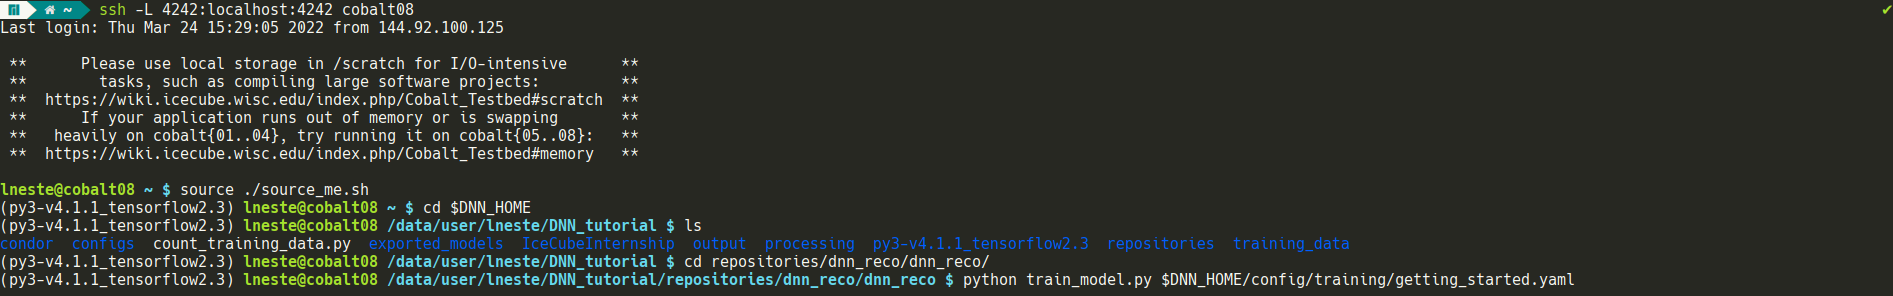
\includegraphics[width=\textwidth]{media/console.png}
\end{frame}
\begin{frame}{A First Model @13000 Training Iterations}
    \begin{columns}
        \begin{column}{.35\textwidth}
            \begin{tabular}{>{\small\bf}r l}
                \toprule
                Features                  & 9                \\
                Batch Size                & 32               \\
                UDC conv. layers          & 4                \\
                LDC conv. layers          & 8                \\
                Hex. conv. layers         & 8                \\
                Dense layers              & 1\times50        \\
                $\rightarrow$ Free Params & 24532            \\
                \midrule
                Loss function             & GL               \\
                Optimizer                 & ADAM             \\
                Learning Rate             & $10^{-3}$        \\
                Input Dropout Rate        & \SI{5}{\percent} \\
                \bottomrule
            \end{tabular}
        \end{column}
        \begin{column}{.65\textwidth}
            \begin{figure}
                \centering
                \only<2>{only
                    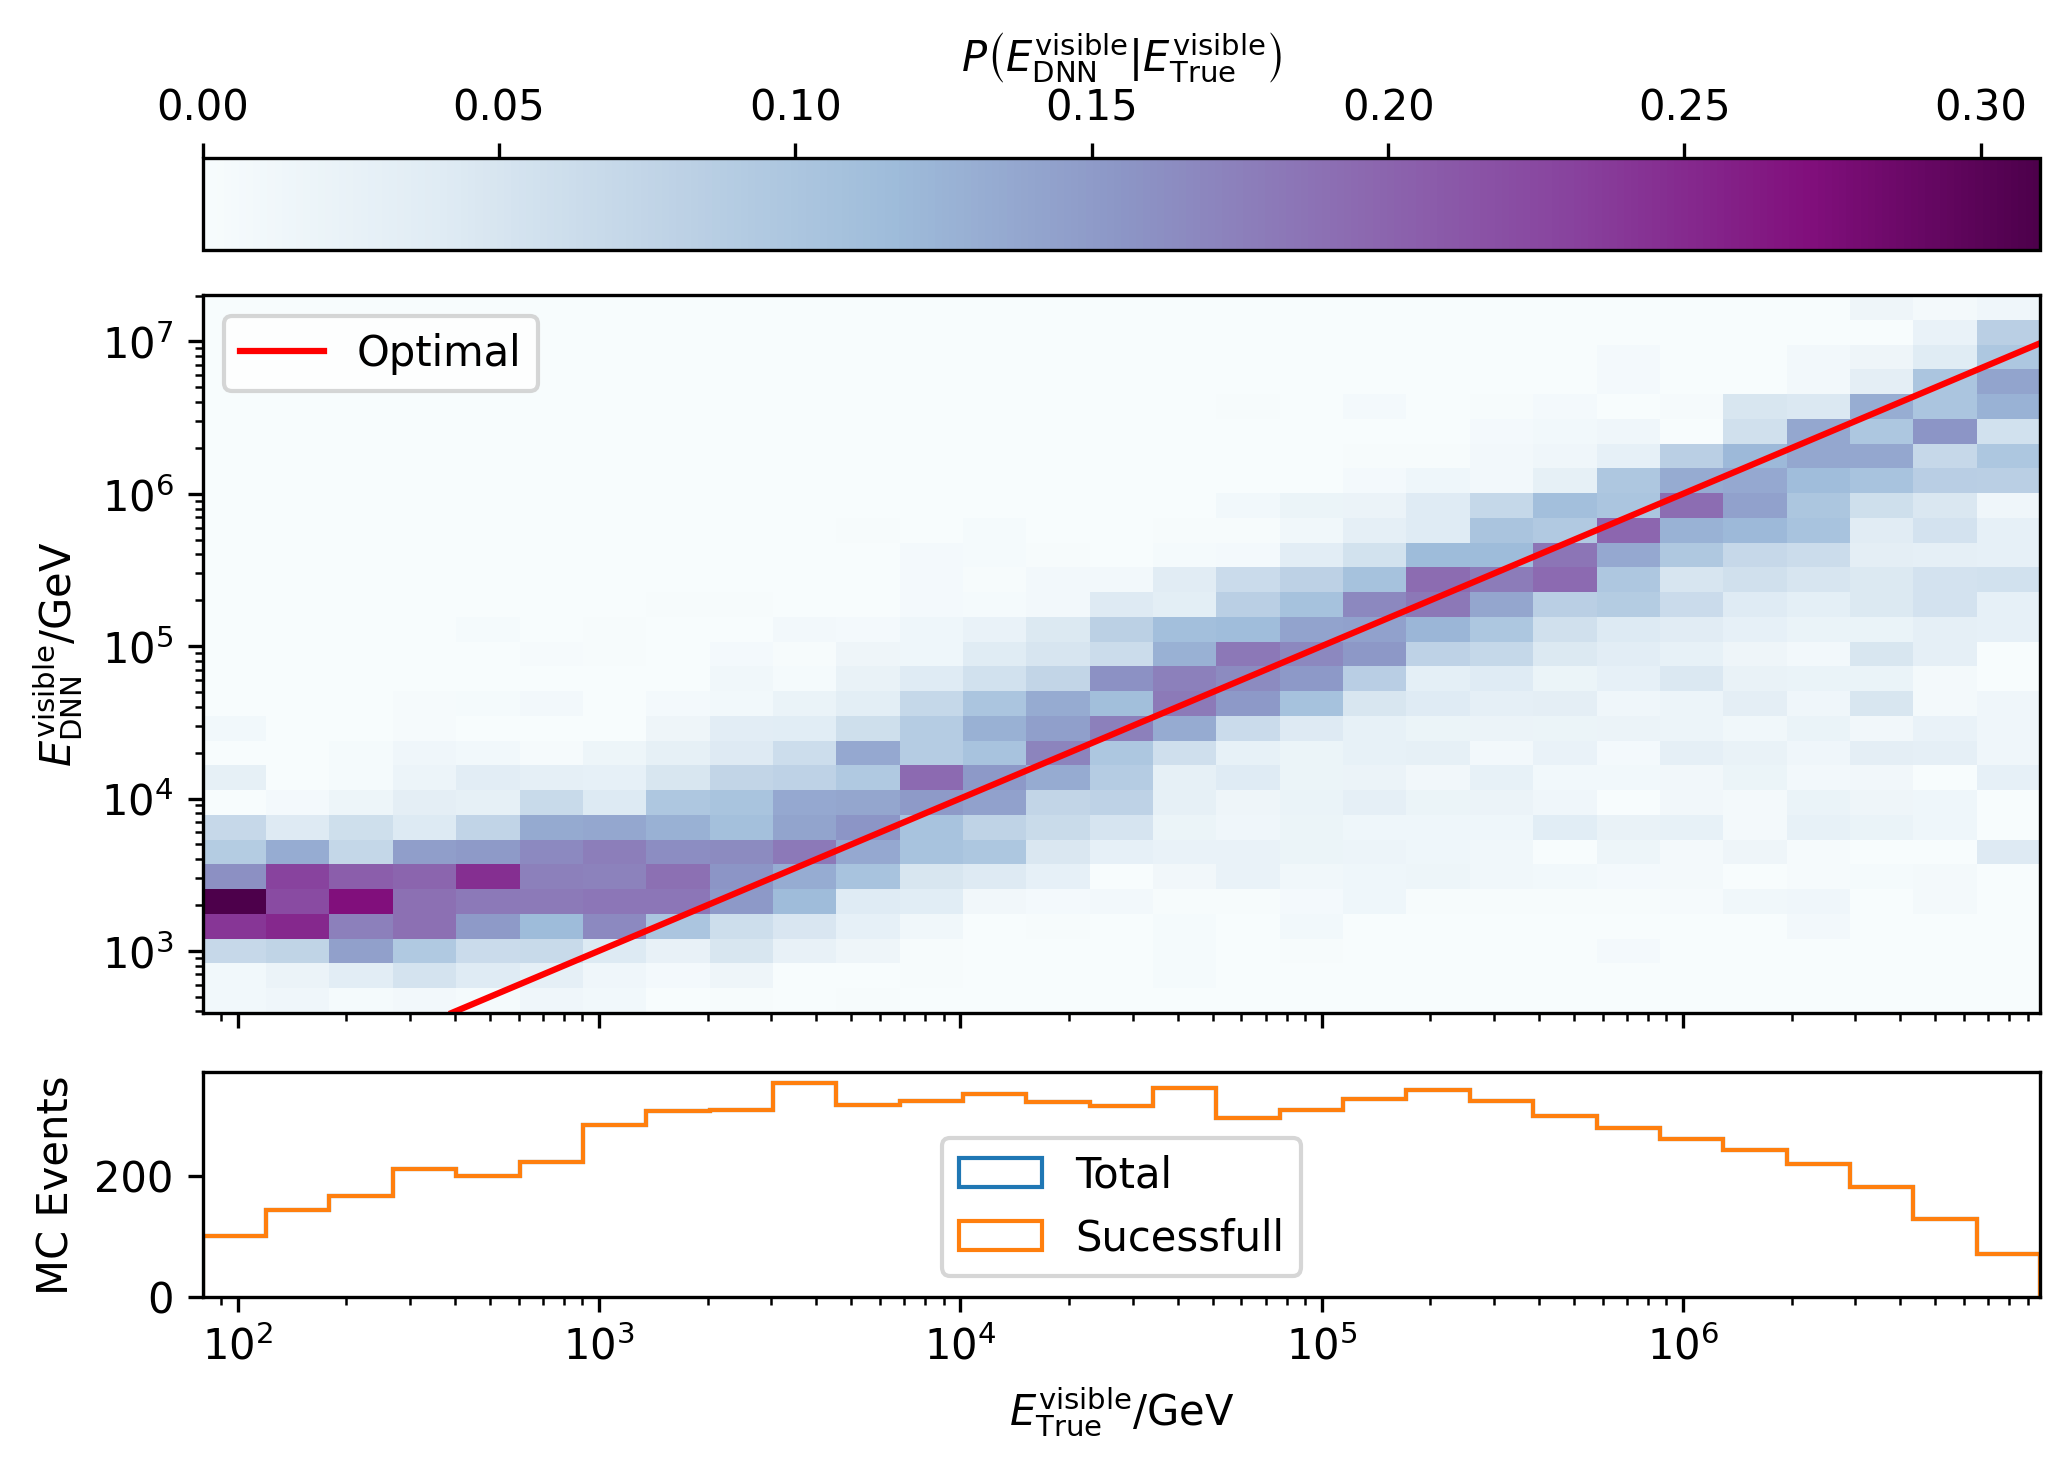
\includegraphics[width=.95\textwidth]{media/DNN_CORR.png}
                    \caption*{\small Normalized correlation plot of visible energy}
                }
                \only<3>{
                    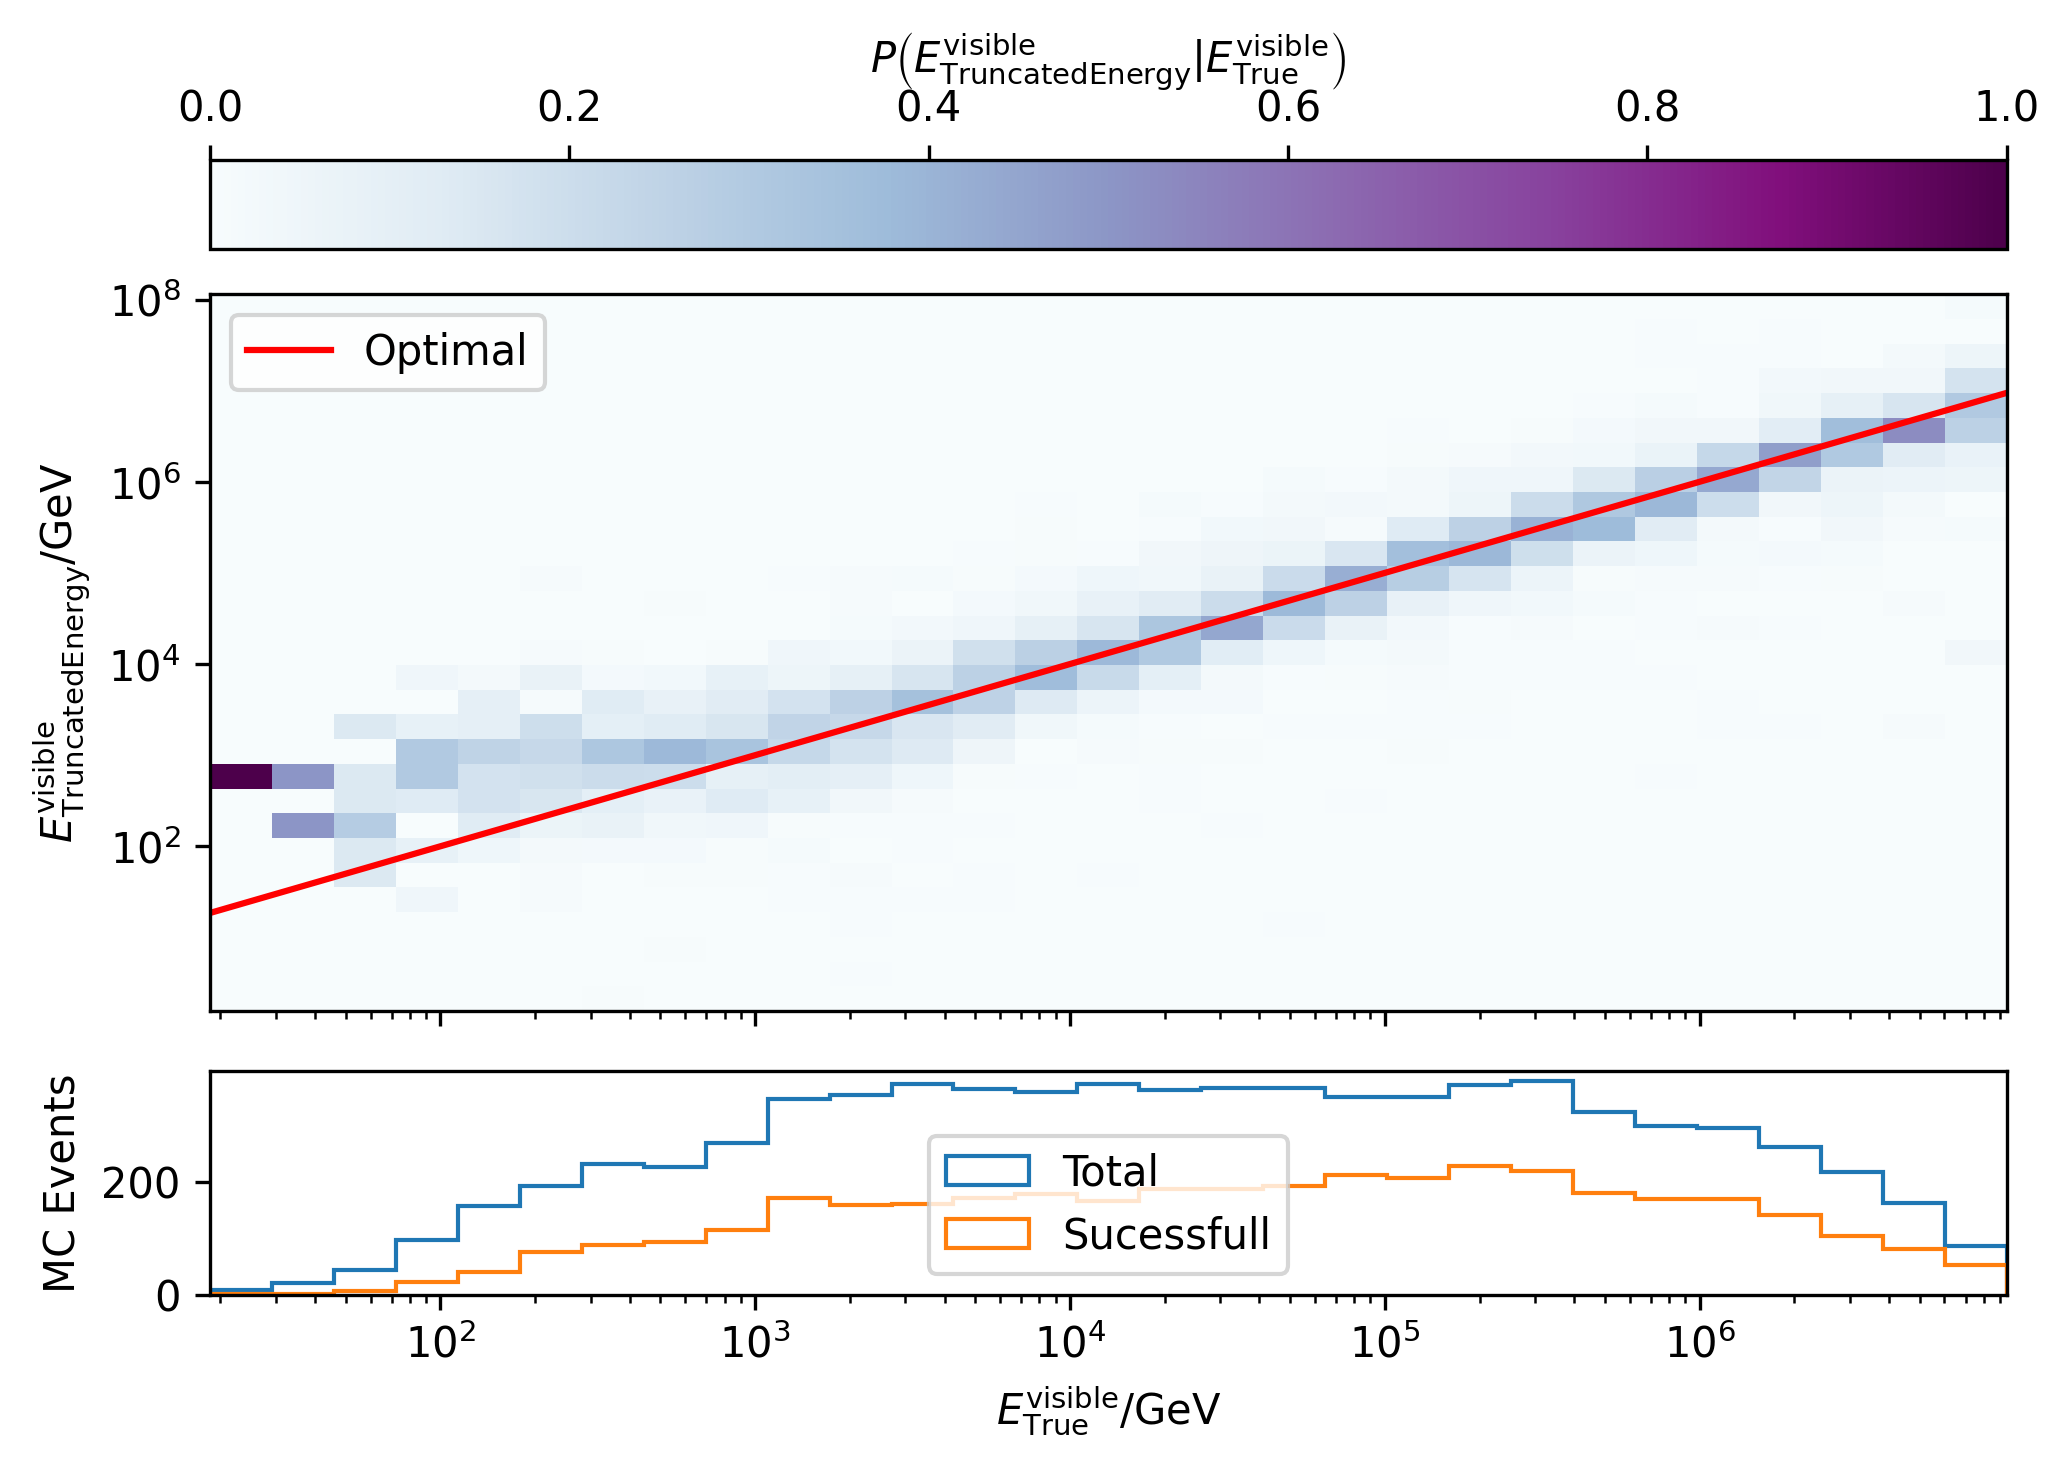
\includegraphics[width=.95\textwidth]{media/TRUN_CORR.png}
                    \caption*{\small Normalized correlation plot of visible energy (truncated energy)}
                }
            \end{figure}
        \end{column}
    \end{columns}
\end{frame}
\begin{frame}{A First Model for Directional Reconstruction \only<2>{@8.5k}\only<3>{@24.5k}\only<4>{@300k}\only<5>{@1.5m}\only<6>{MPEFit}}
    \only<1>{
        \begin{tabular}{>{\small\bf}r l}
            \toprule
            Features                  & 9         \\
            Batch Size                & 32        \\
            UDC conv. layers          & 4         \\
            LDC conv. layers          & 8         \\
            Hex. conv. layers         & 8         \\
            Dense layers              & 1\times50 \\
            $\rightarrow$ Free Params & 24532     \\
            \bottomrule
        \end{tabular}}
    \begin{figure}
        \centering
        \only<2>{
            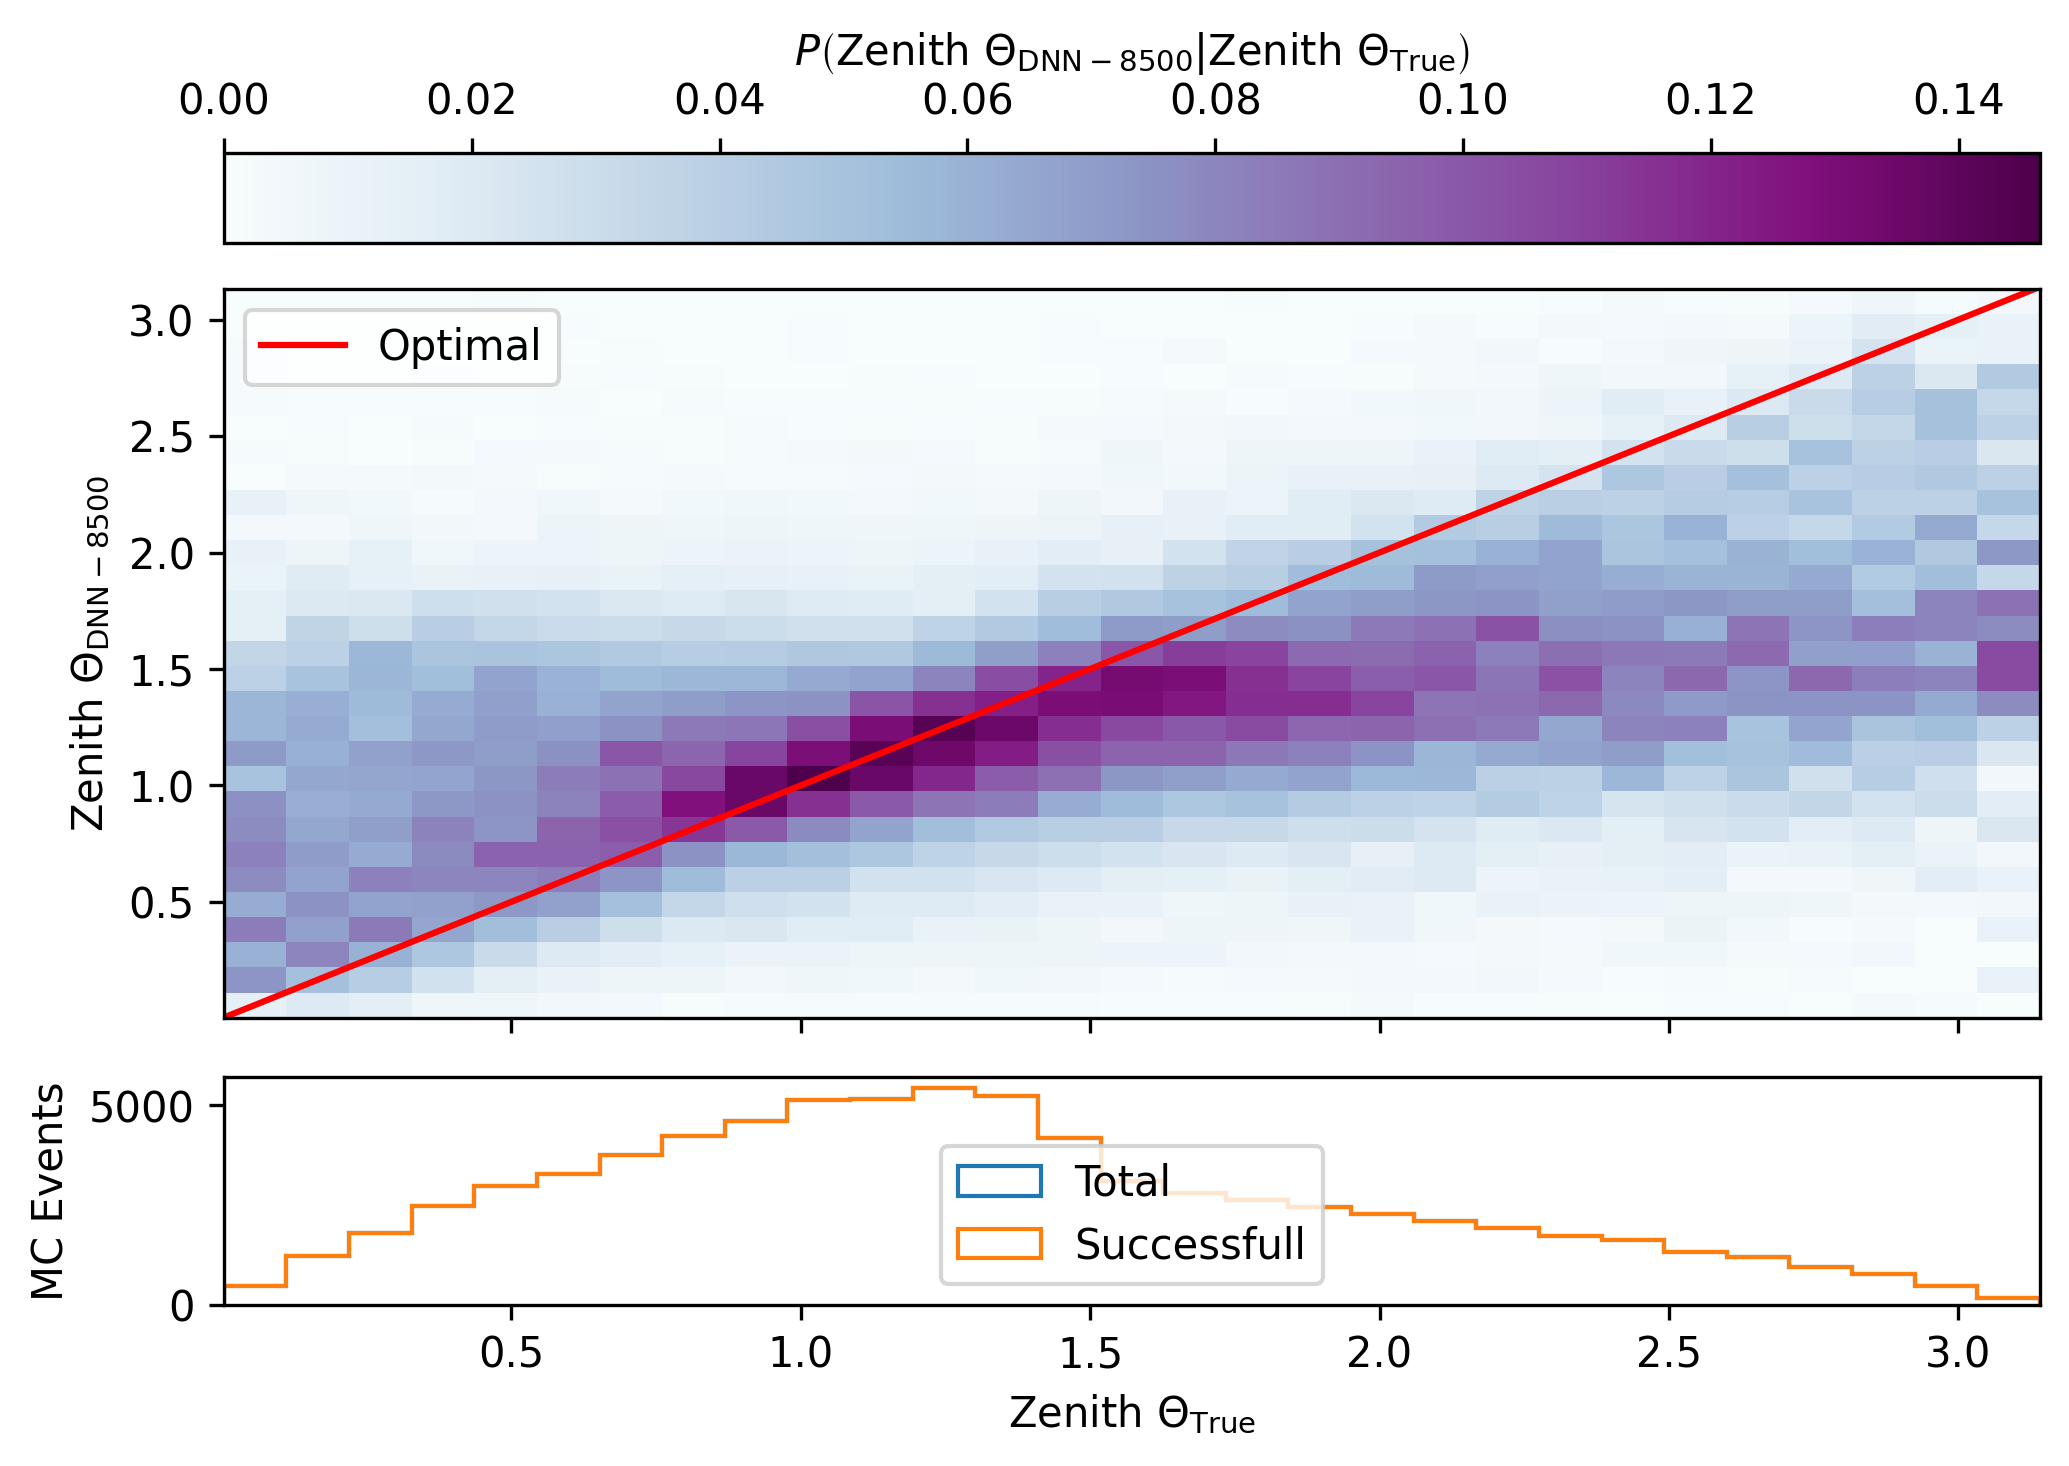
\includegraphics[width=.65\textwidth]{media/zenith_8500.png}
        }
        \only<3>{
            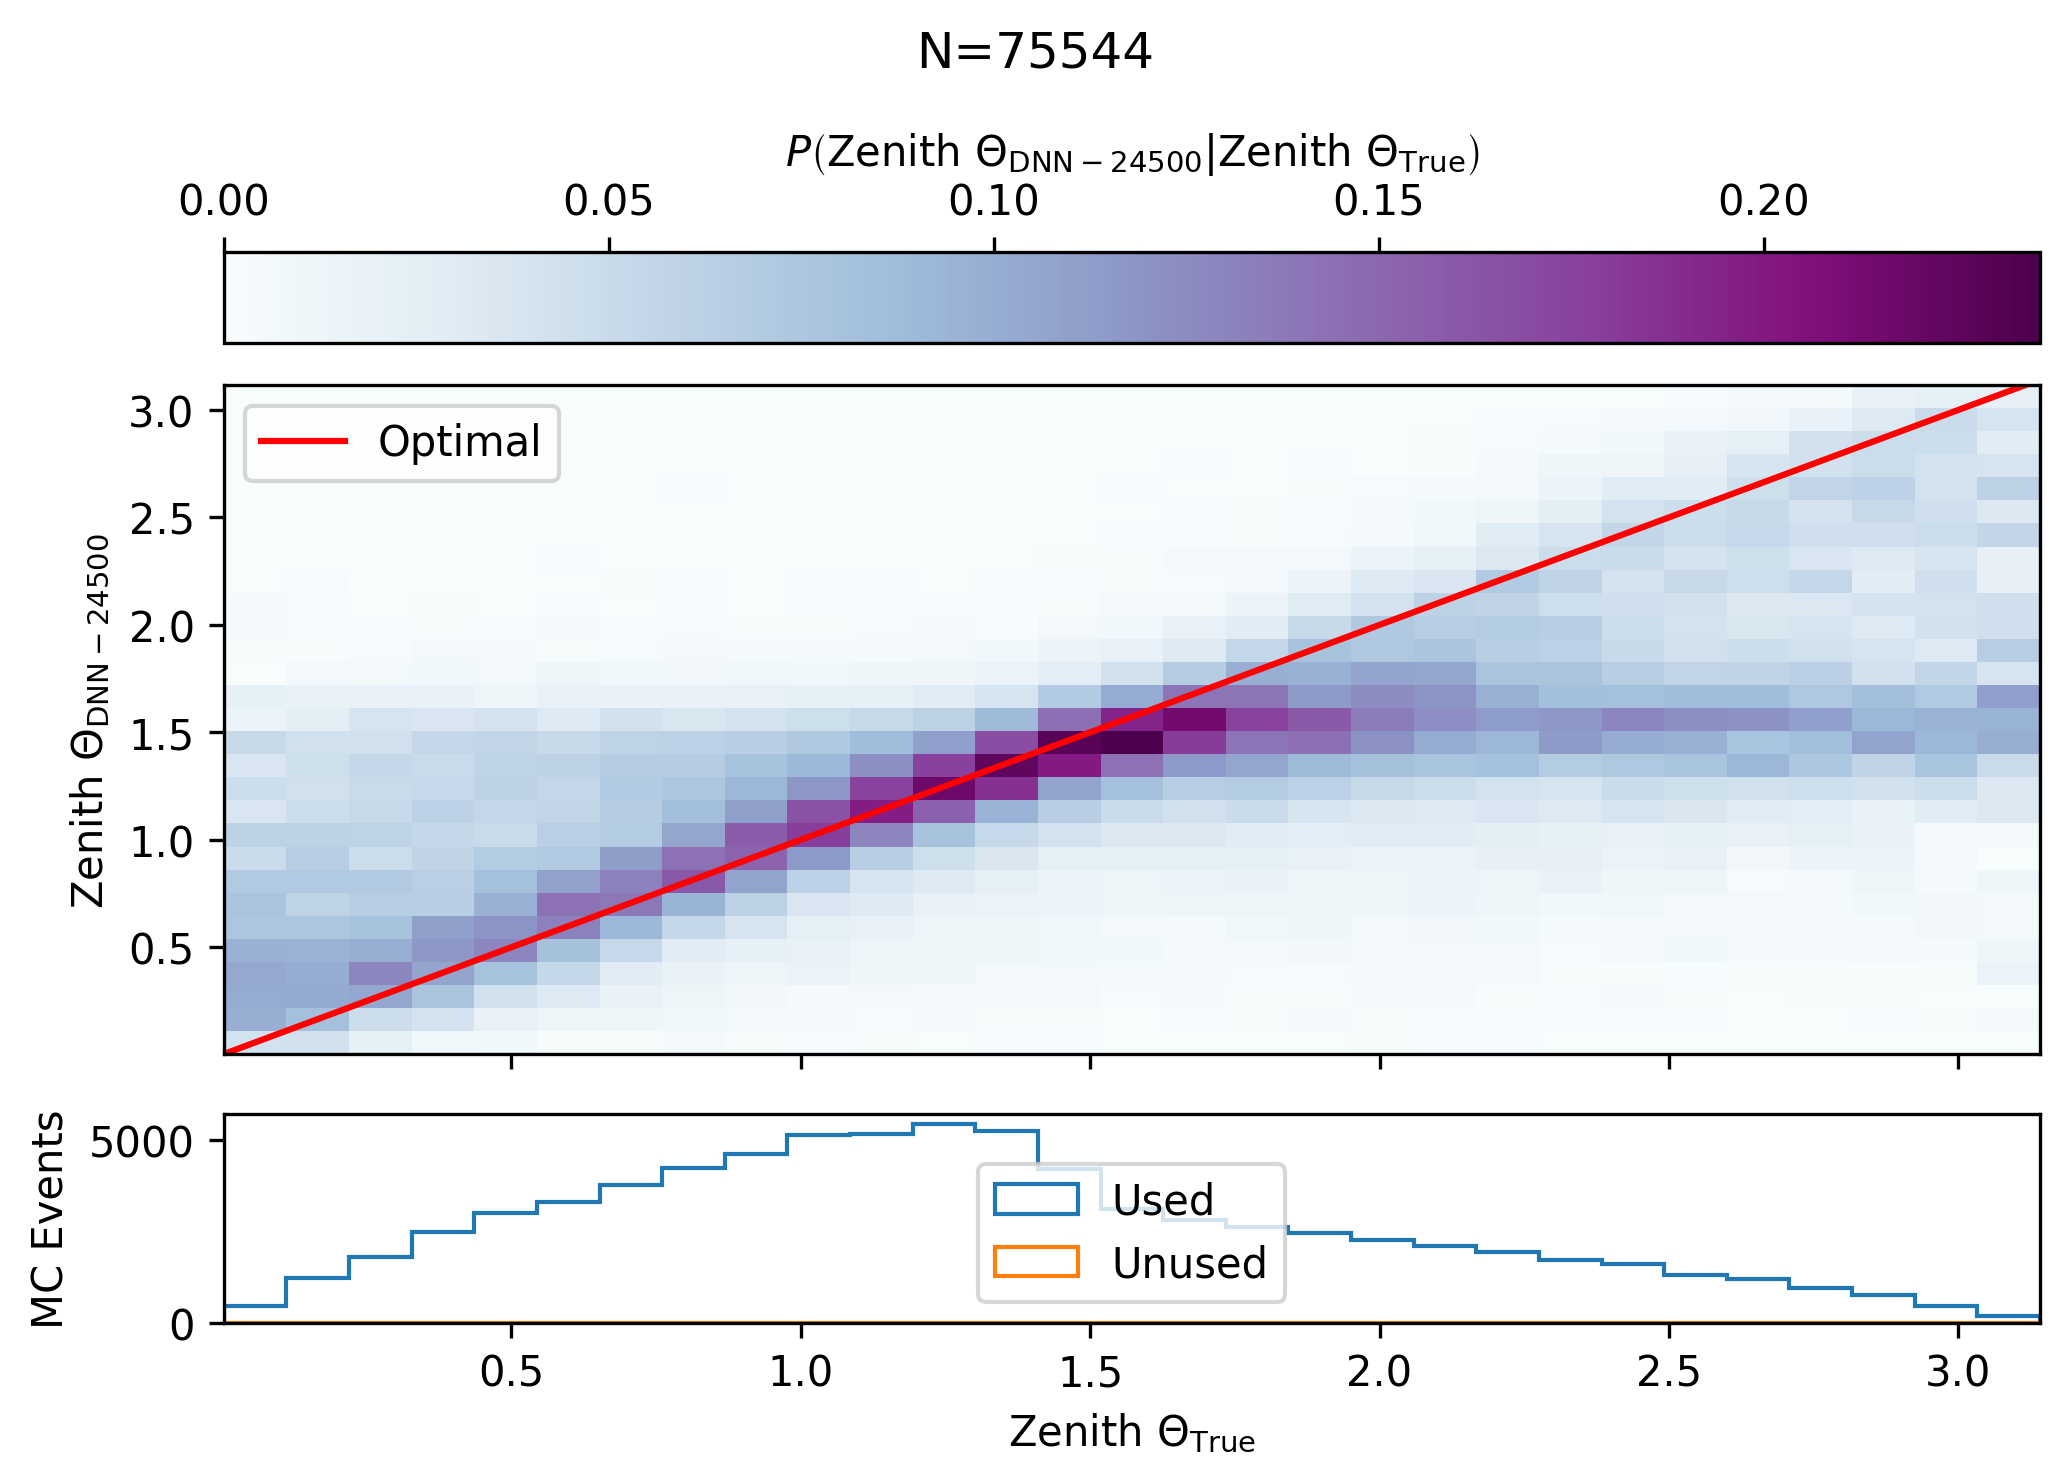
\includegraphics[width=.65\textwidth]{media/zenith_24500.png}
        }
        \only<4>{
            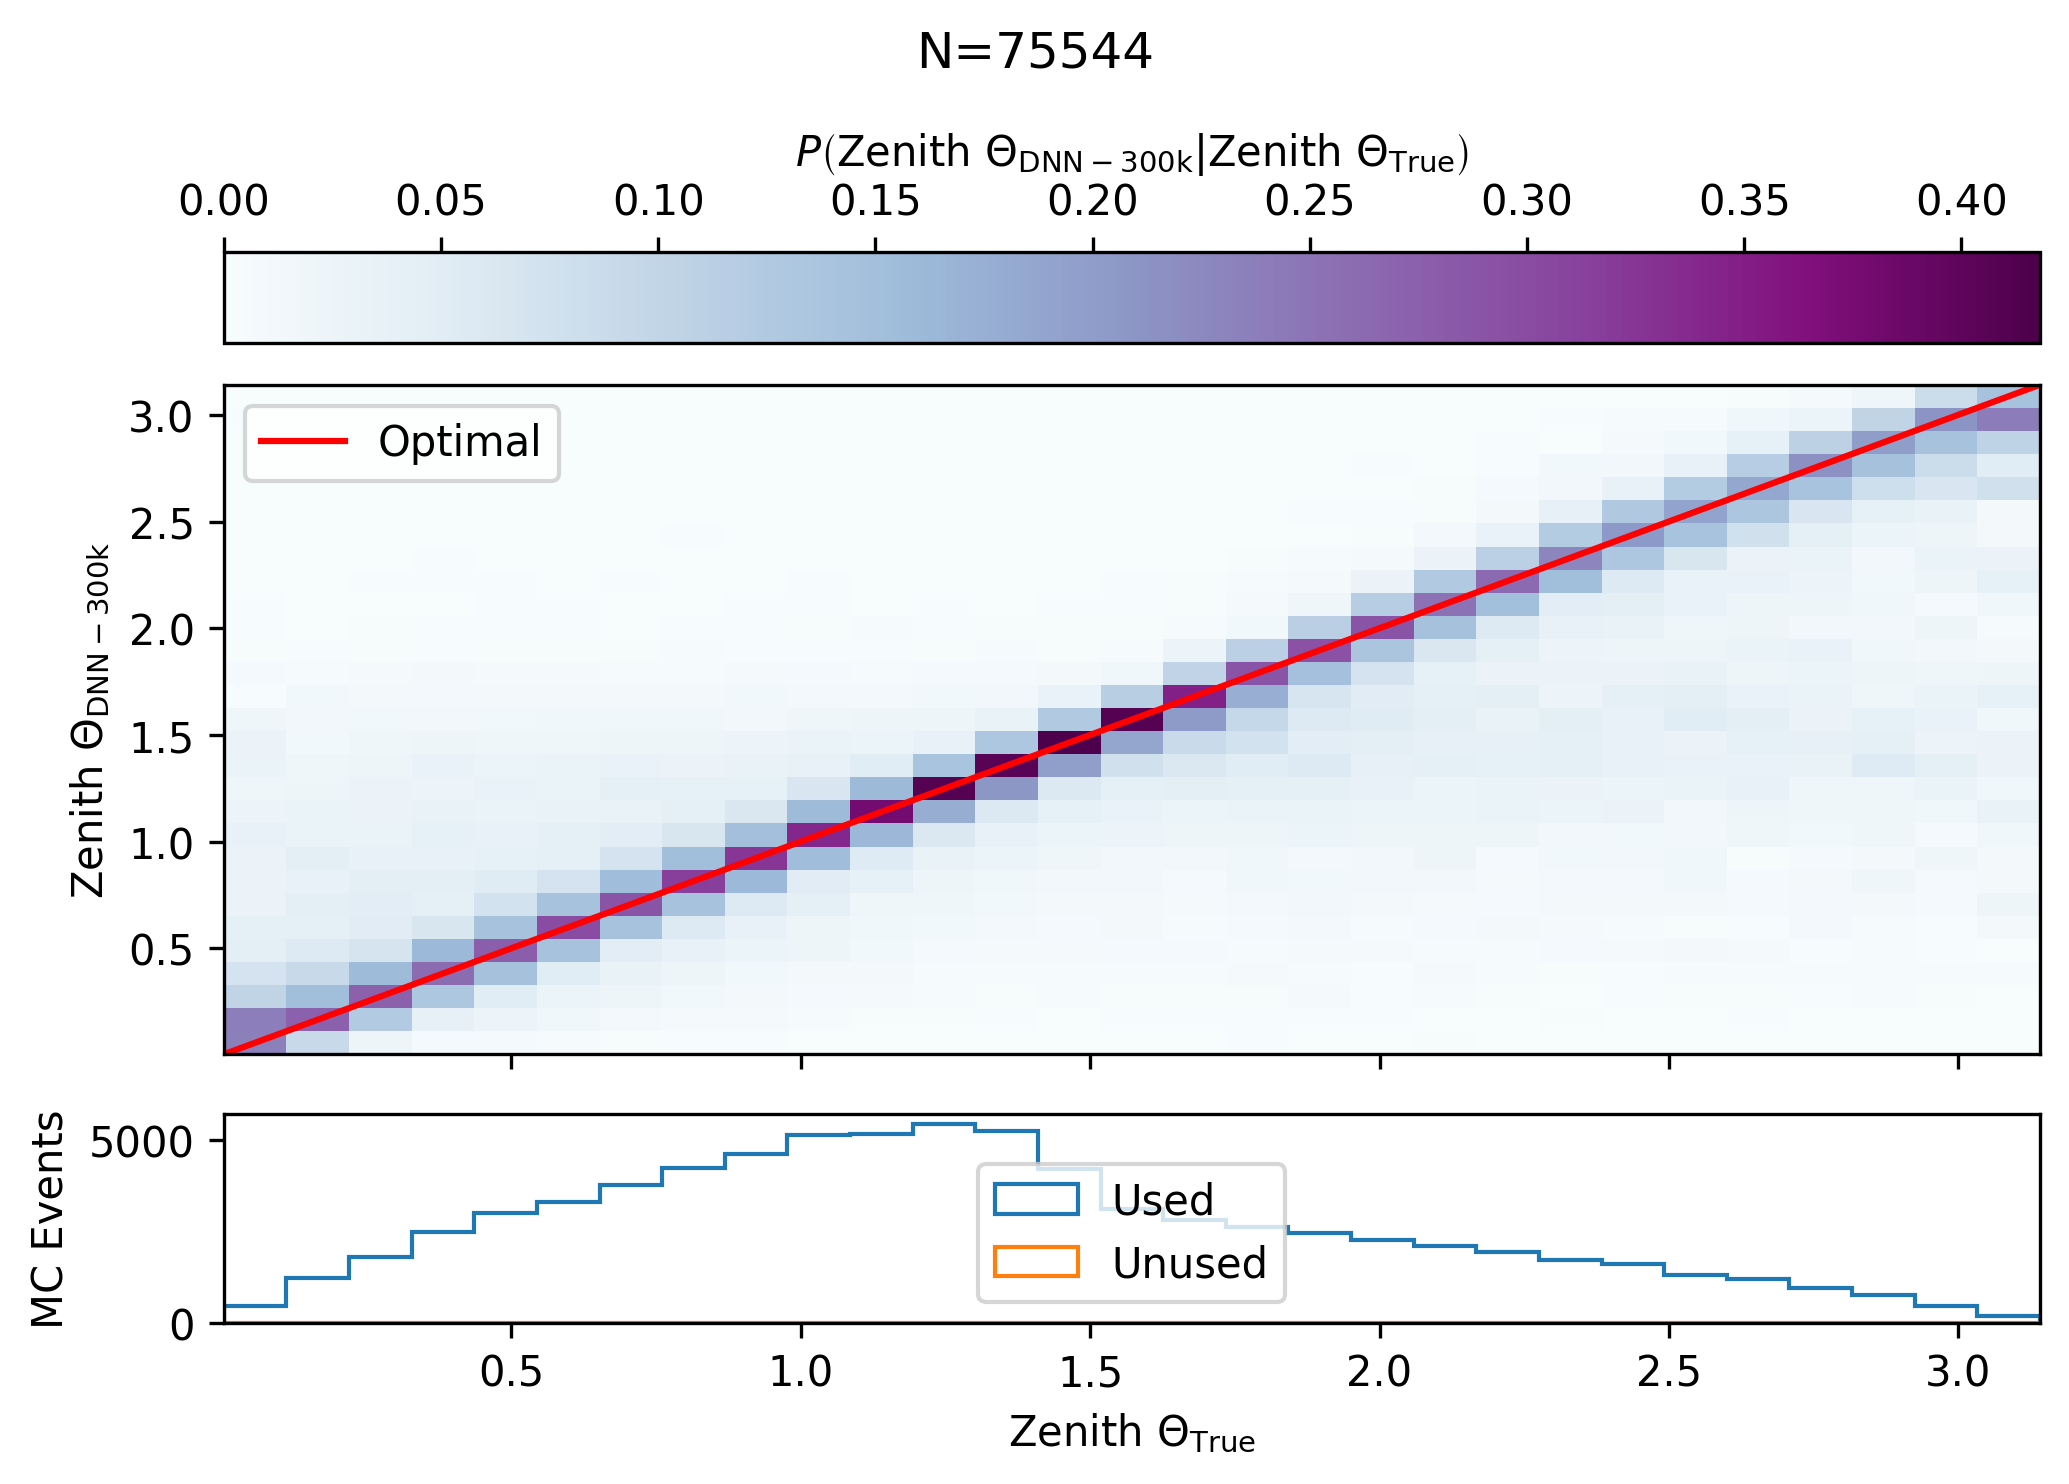
\includegraphics[width=.65\textwidth]{media/zenith_300k.png}
        }
        \only<5>{
            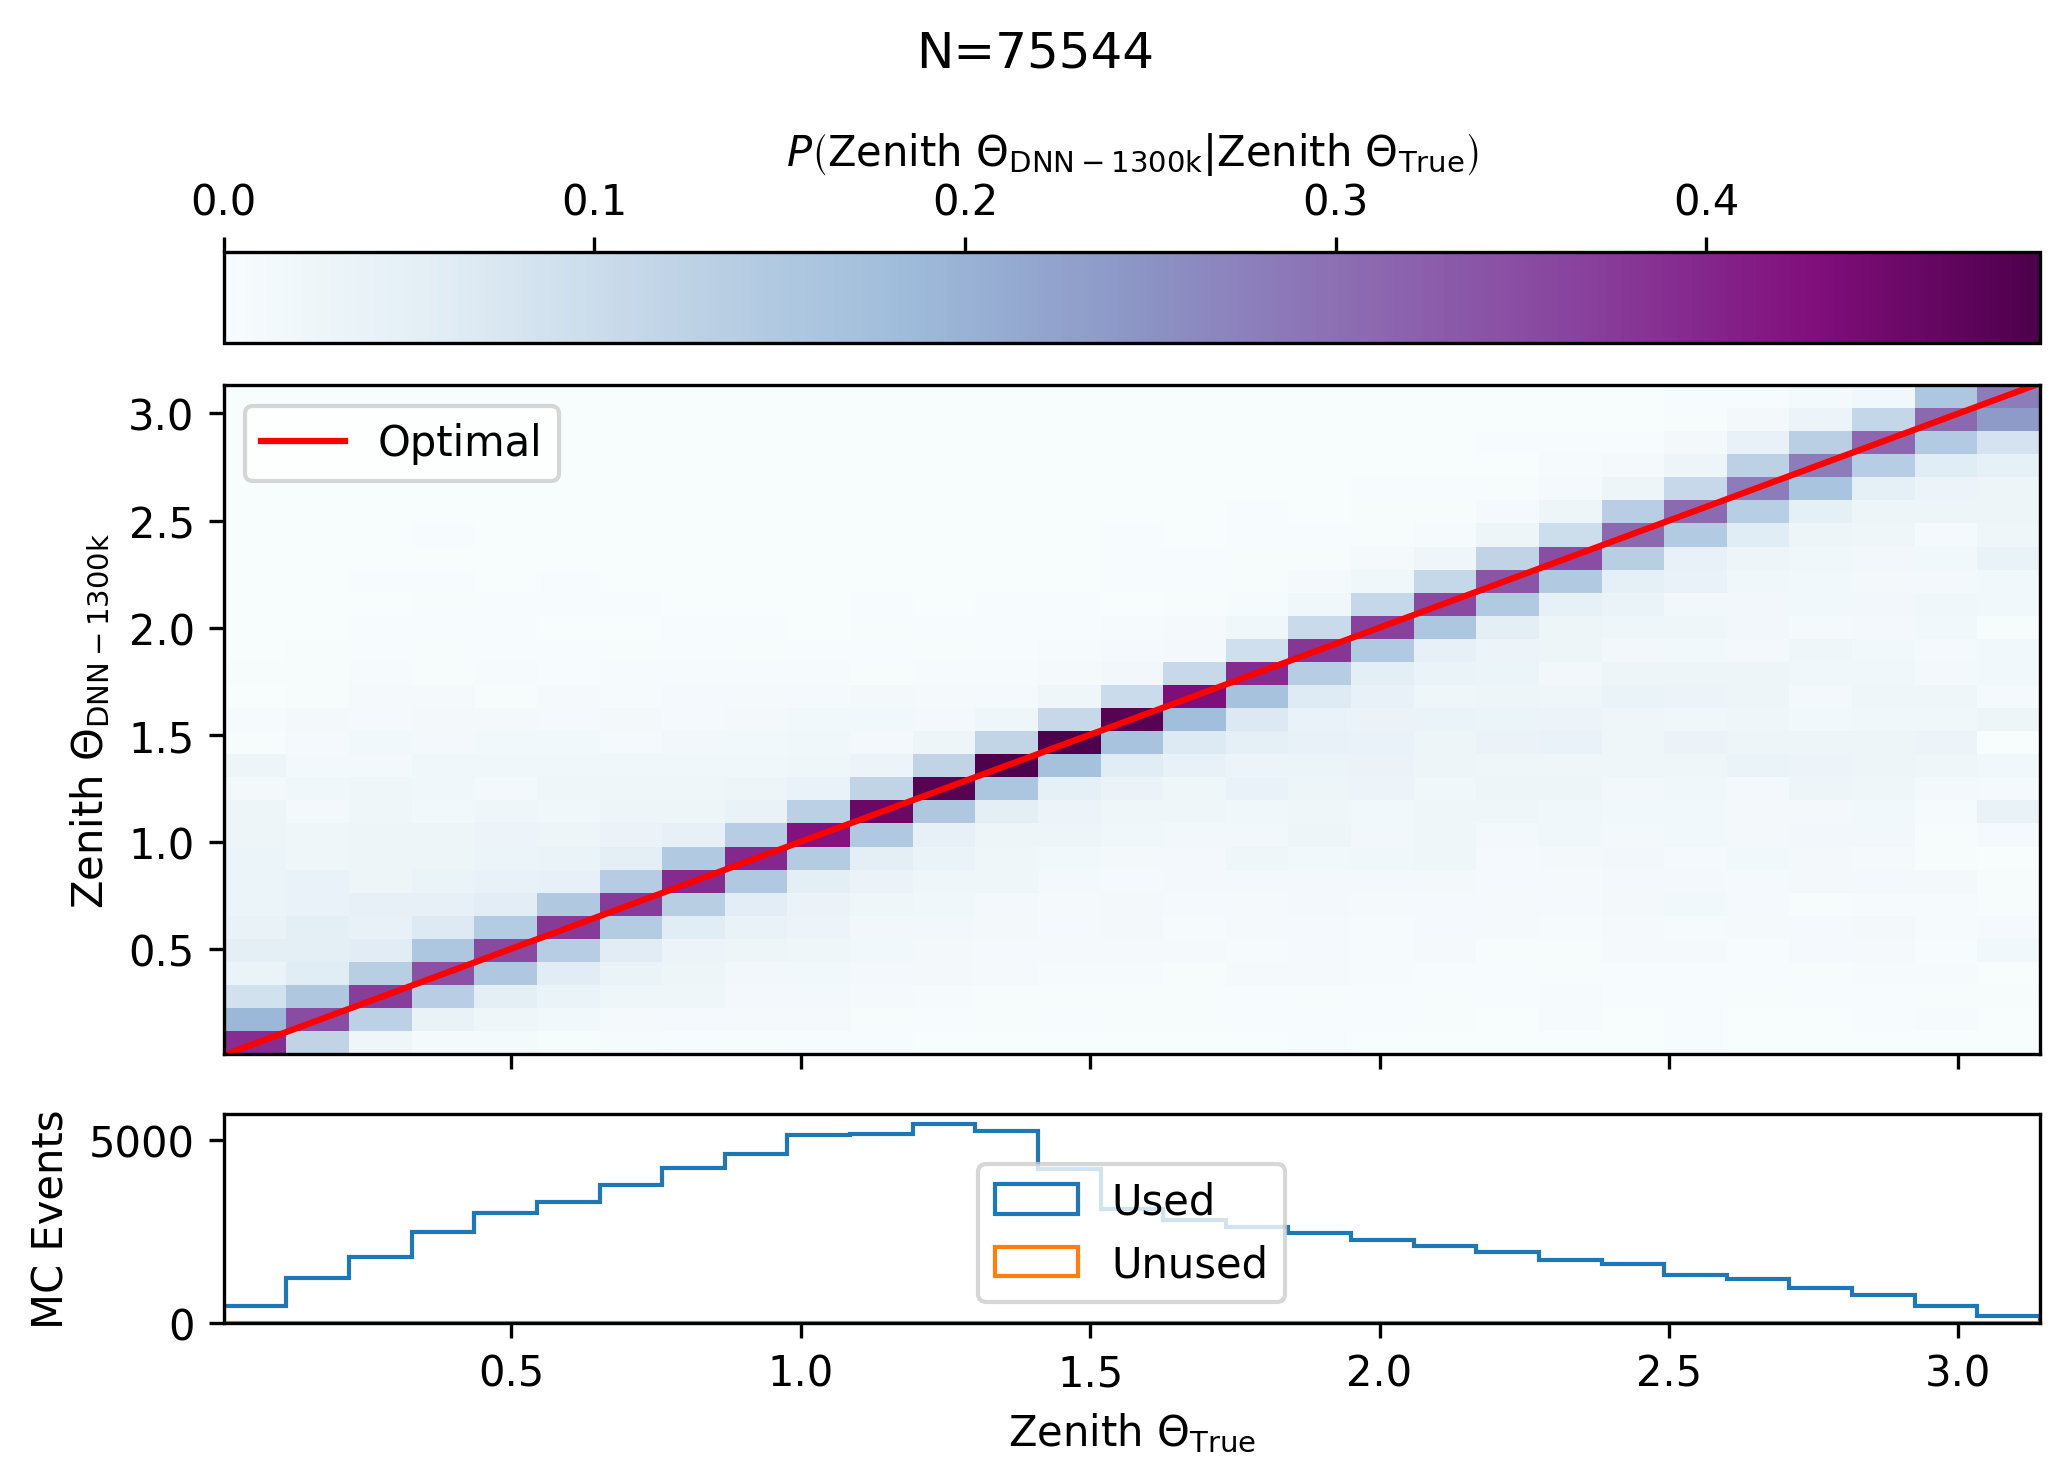
\includegraphics[width=.65\textwidth]{media/zenith_1.5m.png}
        }
        \only<6>{
            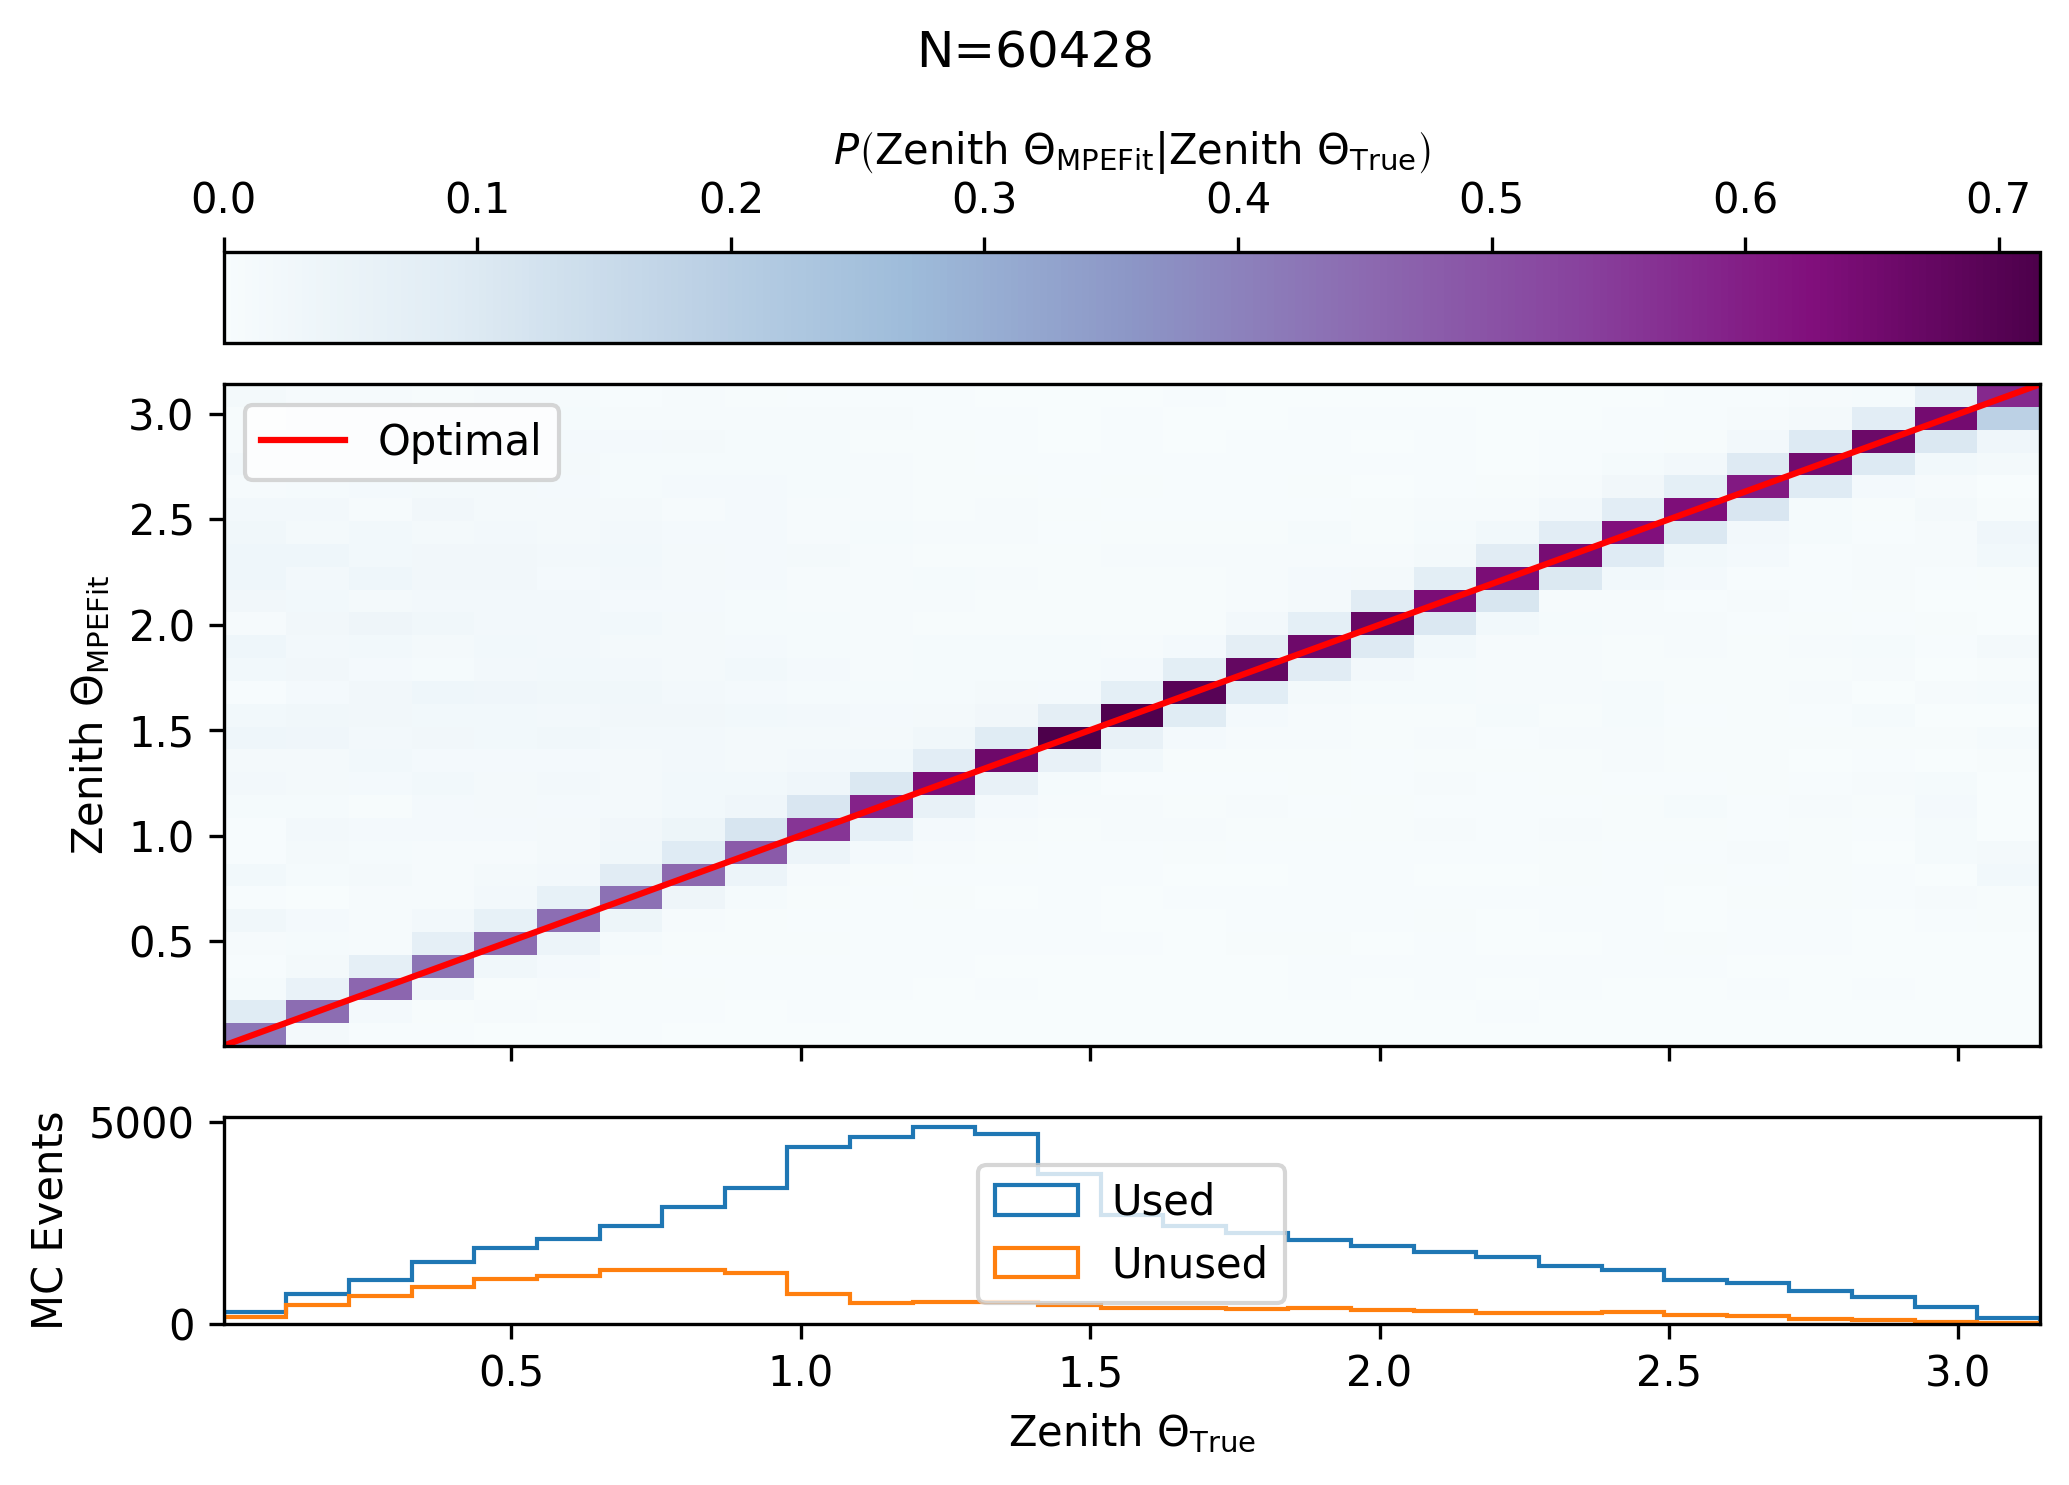
\includegraphics[width=.65\textwidth]{media/zenith_mpefit.png}
        }
        \only<7>{
            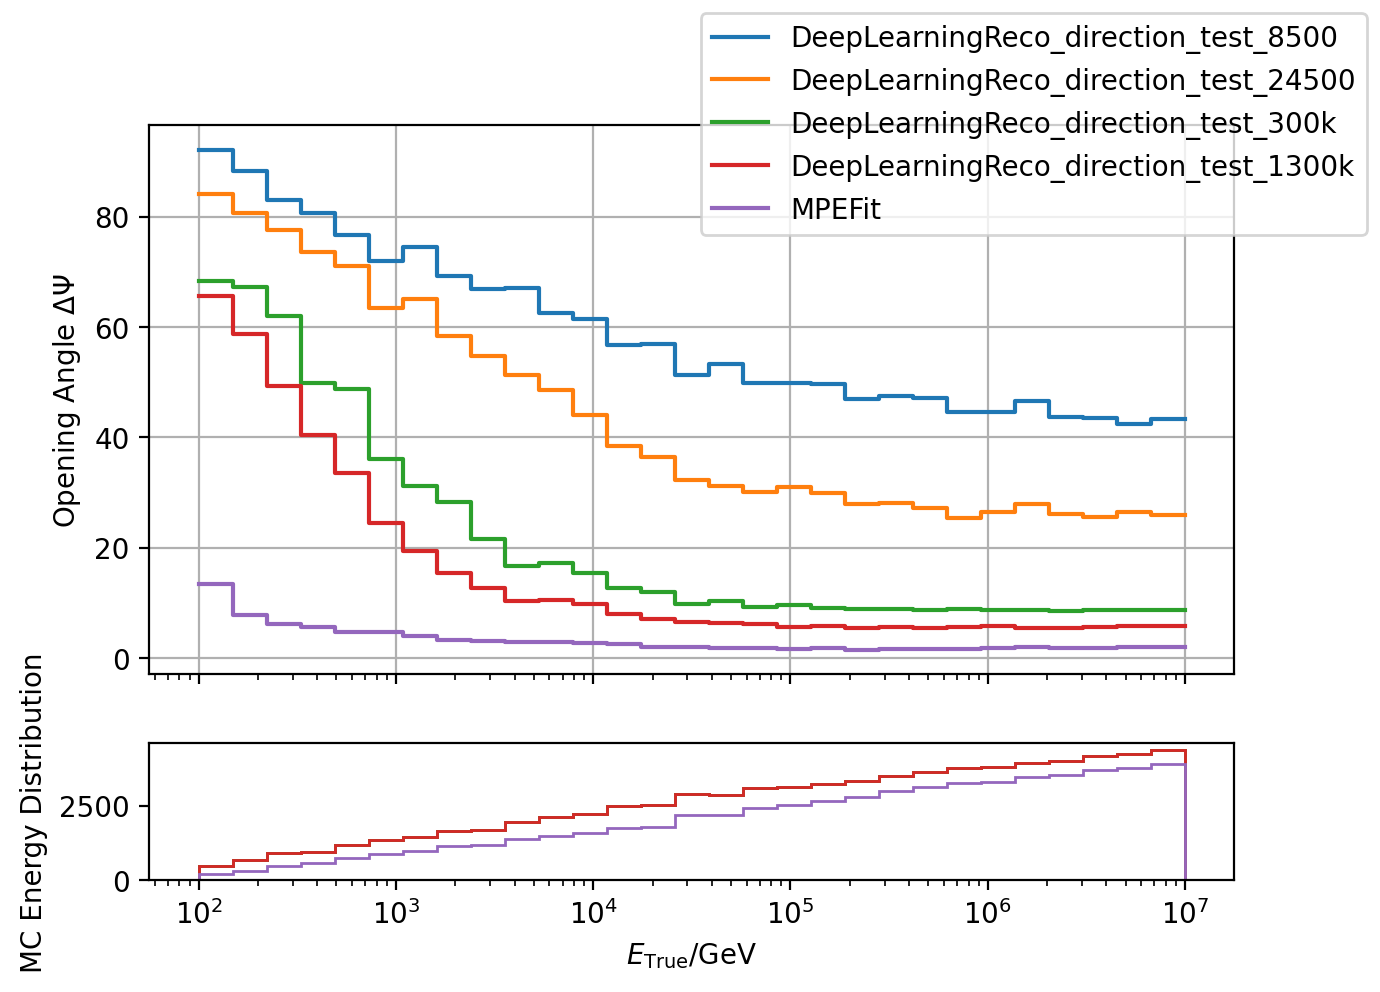
\includegraphics[width=.8\textwidth]{media/getting_started_opening_angle.png}
            % \caption*{\small Median opening angle as a function of $E_\nu$}
        }
    \end{figure}
\end{frame}
\begin{frame}{Improving the Model: Reduced Featureset}
    \begin{columns}
        \begin{column}{.35\textwidth}
            \begin{tabular}{>{\small\bf}r l}
                \toprule
                Features                  & 3         \\
                Batch Size                & 64        \\
                UDC conv. layers          & 4         \\
                LDC conv. layers          & 8         \\
                Hex. conv. layers         & 8         \\
                Dense layers              & 1\times50 \\
                $\rightarrow$ Free Params & 22462     \\
                \bottomrule
            \end{tabular}
        \end{column}
        \begin{column}{.65\textwidth}
            \only<1>{
                \begin{itemize}
                    \item 2070 parameters less
                    \item One test yielded 5-6 times faster training
                    \item Using
                          \begin{itemize}
                              \item total charge $c_{\mathrm{total}}$
                              \item first hit $t_{\mathrm{first}}$
                              \item charge weighted time std $t_{\mathrm{std}}$
                          \end{itemize}
                \end{itemize}
            }
            \only<2>{
                \begin{figure}
                    \centering
                    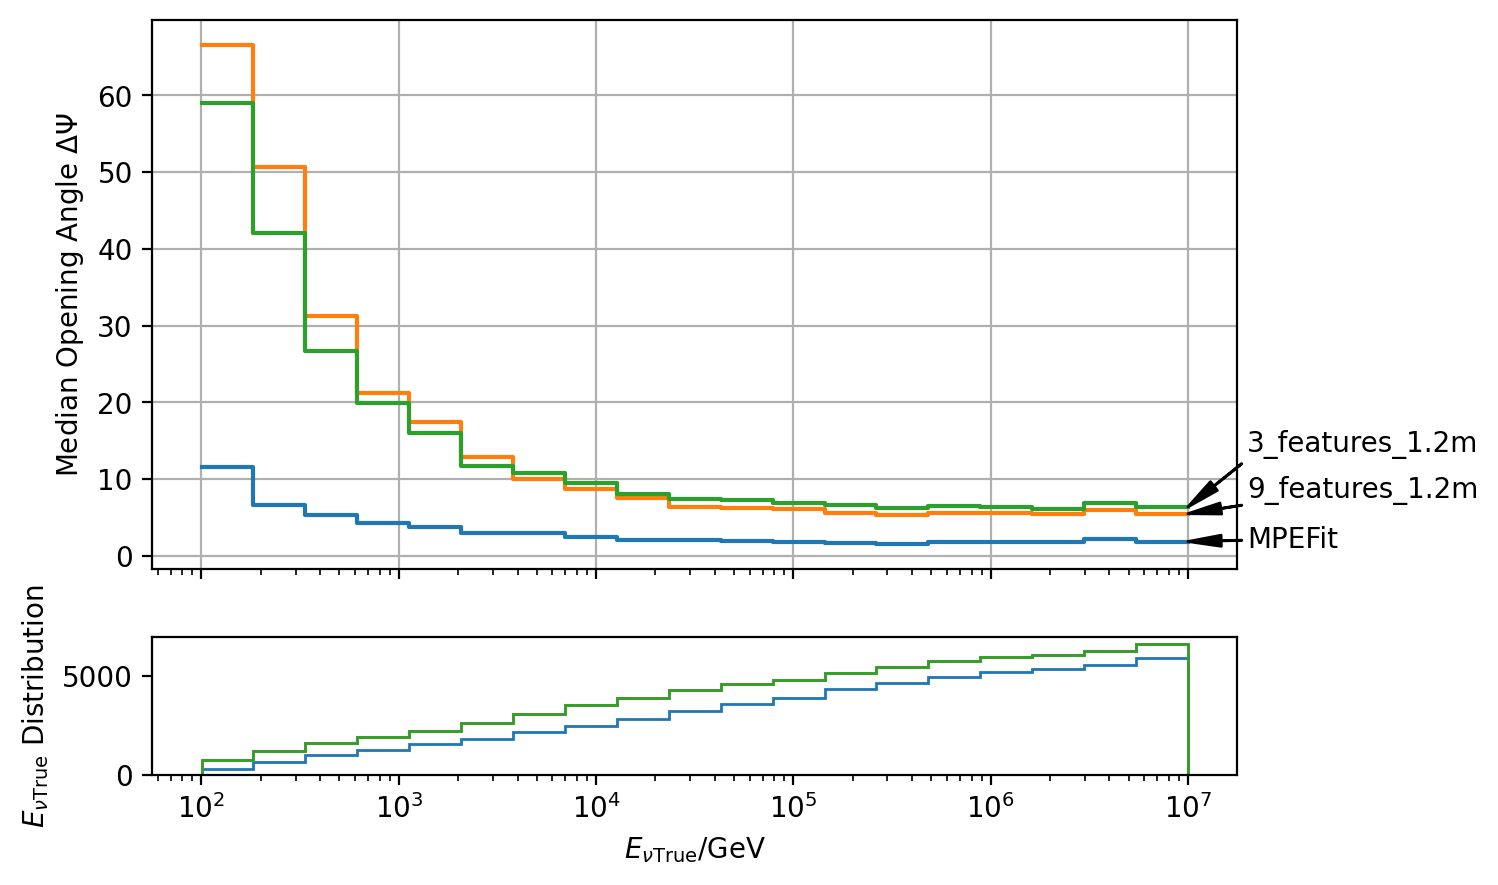
\includegraphics[width=\textwidth]{media/3_vs_9.png}
                    % \caption*{\small Median opening angle as a function of $E_\nu$}
                \end{figure}}
        \end{column}
    \end{columns}
\end{frame}
\begin{frame}{Improving the Model: Higher Complexity}
    \begin{columns}
        \begin{column}{.35\textwidth}
            \begin{tabular}{>{\small\bf}r >{\tiny}r<{\hspace{-2em}} l}
                \toprule
                Features                  &                            & 3                             \\
                Batch Size                &                            & 64                            \\
                UDC conv. lyrs            &                            & 4                             \\
                LDC conv. lyrs            & {8 $\rightarrow$}          & \color{mLightBrown}4          \\
                Hex. conv. lyrs           & {8 $\rightarrow$}          & \color{mLightBrown}9          \\
                Dense layers              & {$1\times 50 \rightarrow$} & \color{mLightBrown}2\times100 \\
                $\rightarrow$ Free Params & {22462 $\rightarrow$}      & {\color{mLightBrown}339467}   \\
                \bottomrule
            \end{tabular}
        \end{column}
        \begin{column}{.65\textwidth}
            \only<1>{
                \begin{figure}
                    \centering
                    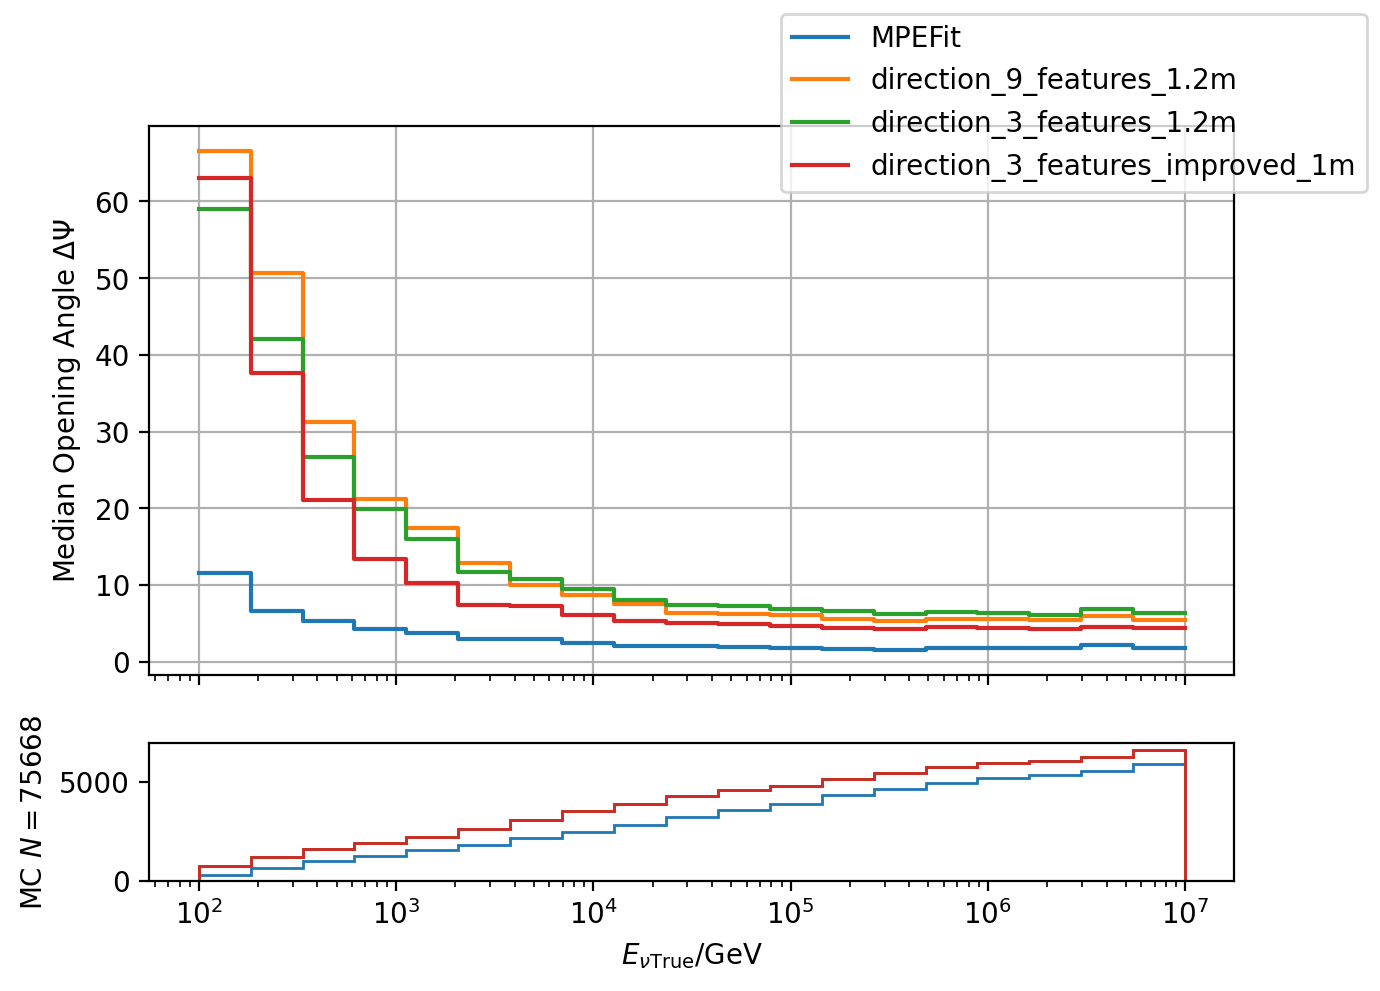
\includegraphics[width=\textwidth]{media/improved_model_compare.png}
                    % \caption*{\small Median opening angle as a function of $E_\nu$}
                \end{figure}}
        \end{column}
    \end{columns}
\end{frame}
\begin{frame}{Improving the Model: Highest Complexity}
    \begin{columns}
        \begin{column}{.35\textwidth}
            \begin{tabular}{>{\small\bf}r >{\tiny}r<{\hspace{-2em}} l}
                \toprule
                Features                  &                             & 3                             \\
                Batch Size                &                             & 64                            \\
                UDC conv. lyrs            & {4 $\rightarrow$}           & \color{mLightBrown}8          \\
                LDC conv. lyrs            & {4 $\rightarrow$}           & \color{mLightBrown}14         \\
                Hex. conv. lyrs           & {9 $\rightarrow$}           & \color{mLightBrown}20         \\
                Dense layers              & {$2\times 100 \rightarrow$} & \color{mLightBrown}2\times300 \\
                $\rightarrow$ Free Params & {339467 $\rightarrow$}      & \color{mLightBrown}5030912    \\
                \bottomrule
            \end{tabular}
        \end{column}
        \begin{column}{.65\textwidth}
            \only<1>{
                \begin{figure}
                    \centering
                    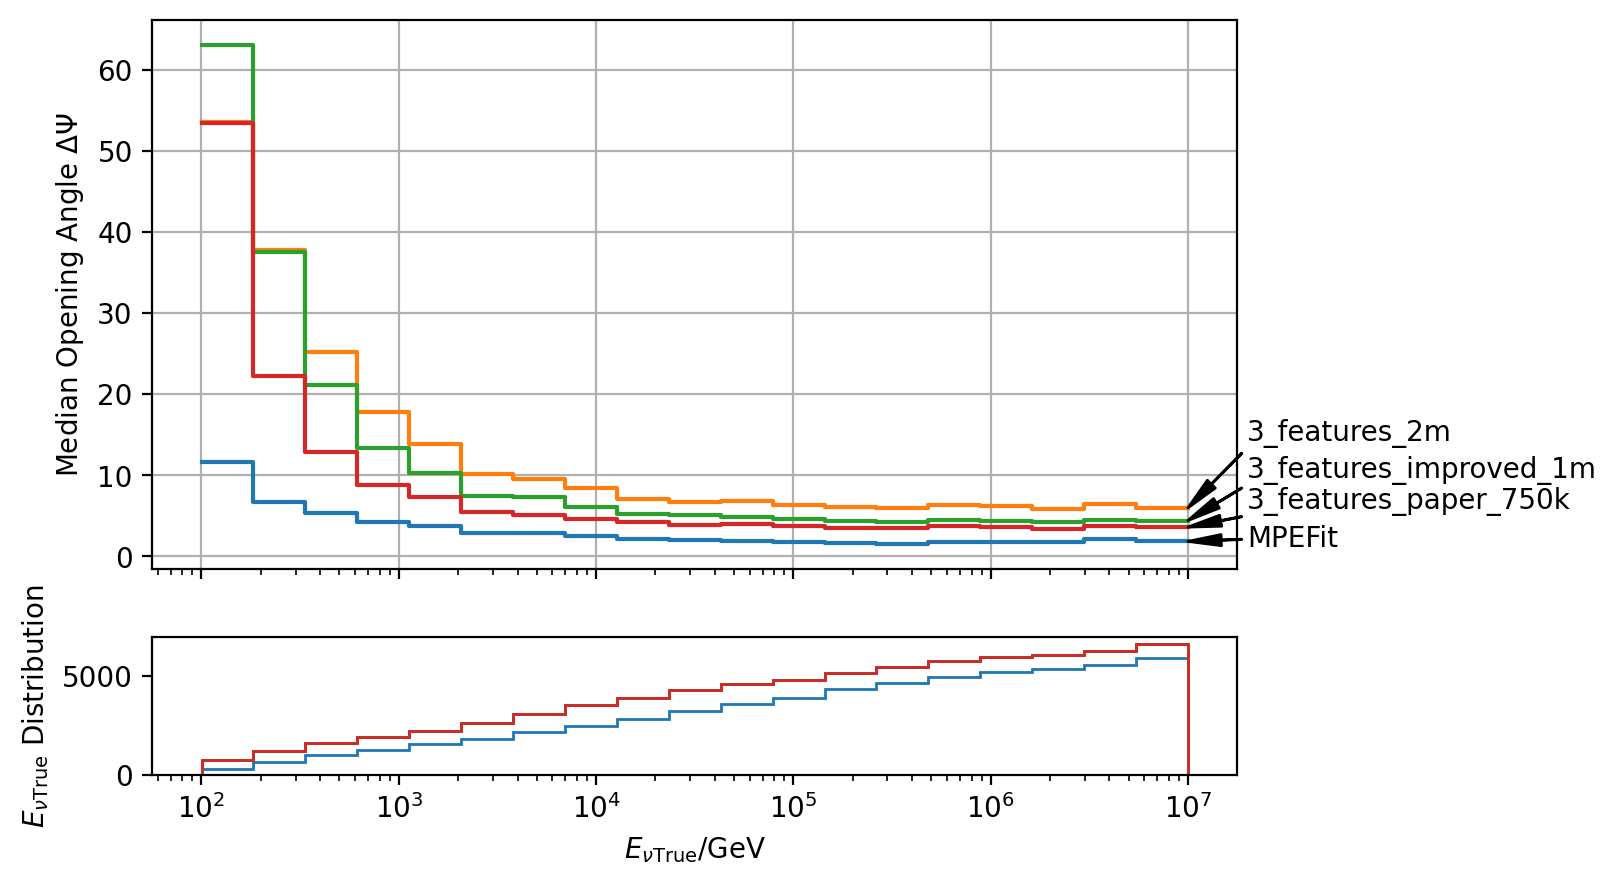
\includegraphics[width=\textwidth]{media/highest_complexity.png}
                \end{figure}}
        \end{column}
    \end{columns}
\end{frame}
\begin{frame}{Uncertainty Estimation with the High Complexity Model}
    \begin{figure}
        \centering
        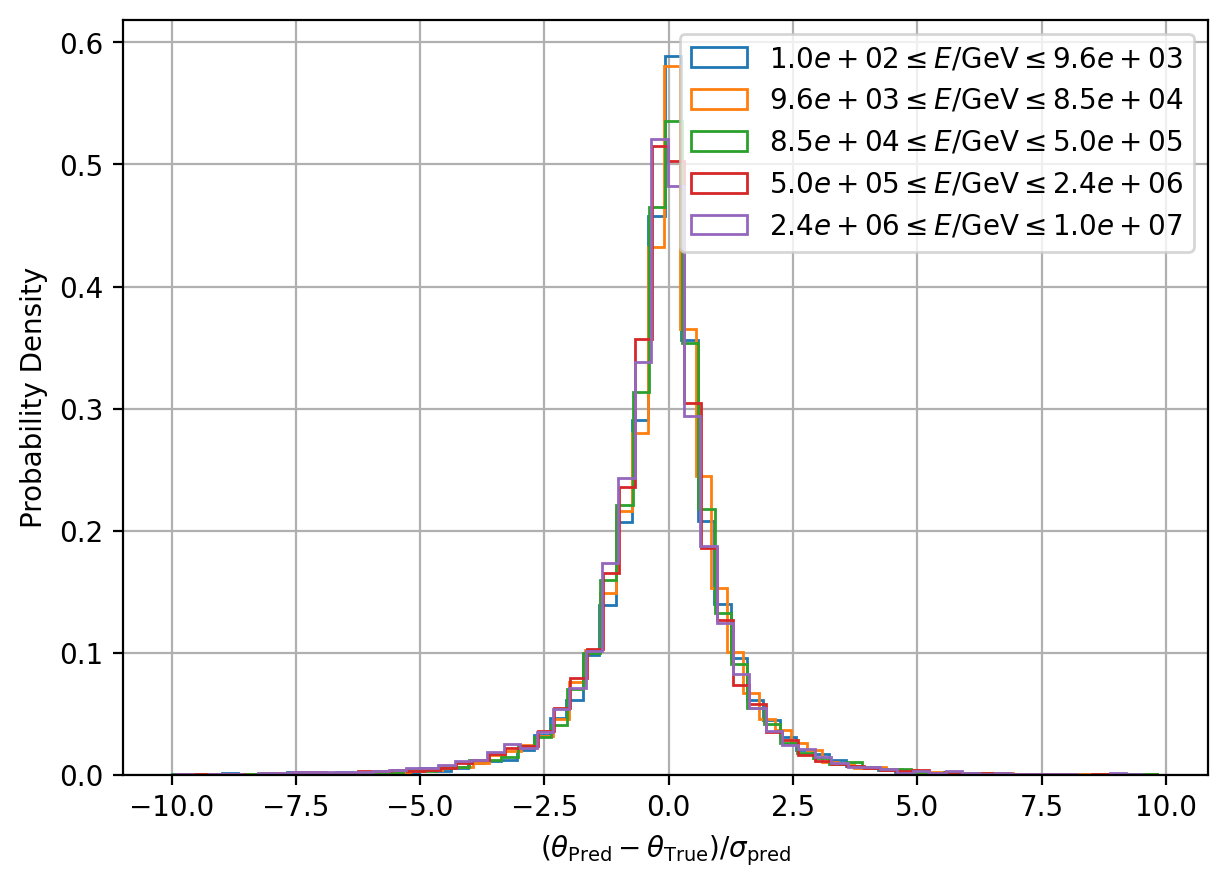
\includegraphics[width=.6\textwidth]{media/pulls.png}
        \caption*{\small Pull plot is peaked compared to expected Gaussian shape, but stable in $E_\nu$}
    \end{figure}
\end{frame}
\begin{frame}{Uncertainty Estimation with the High Complexity Model}
    \begin{figure}
        \centering
        \only<1>{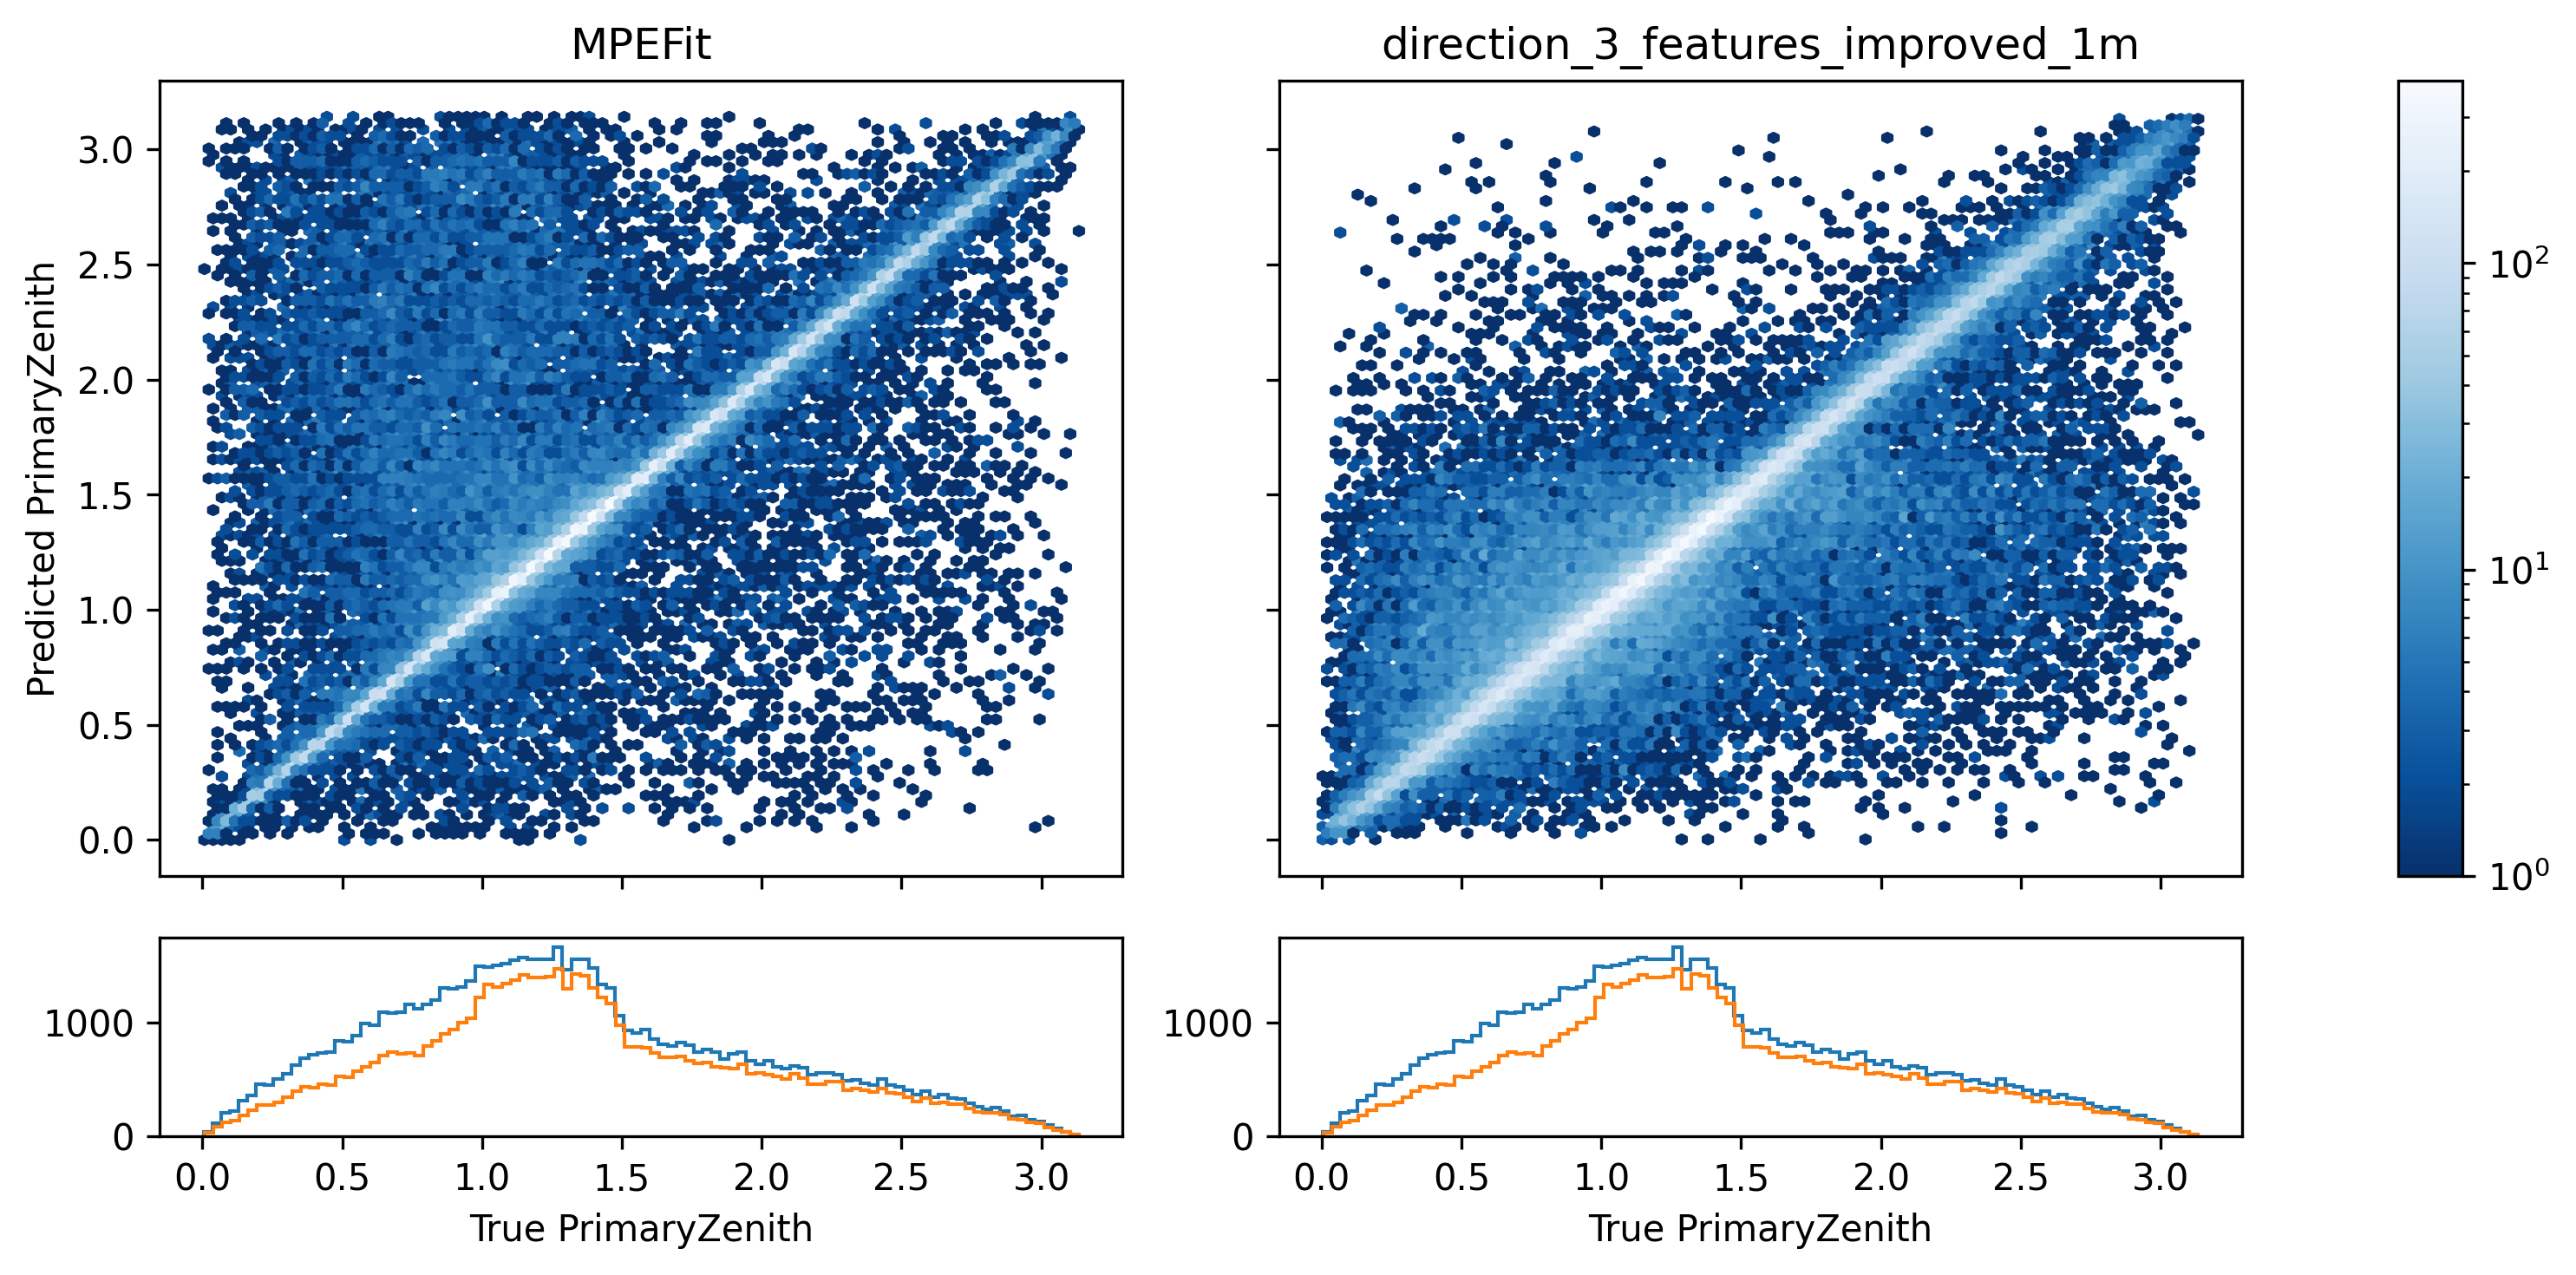
\includegraphics[width=.8\textwidth]{media/scatter_uncertainty.png}}
        \only<2>{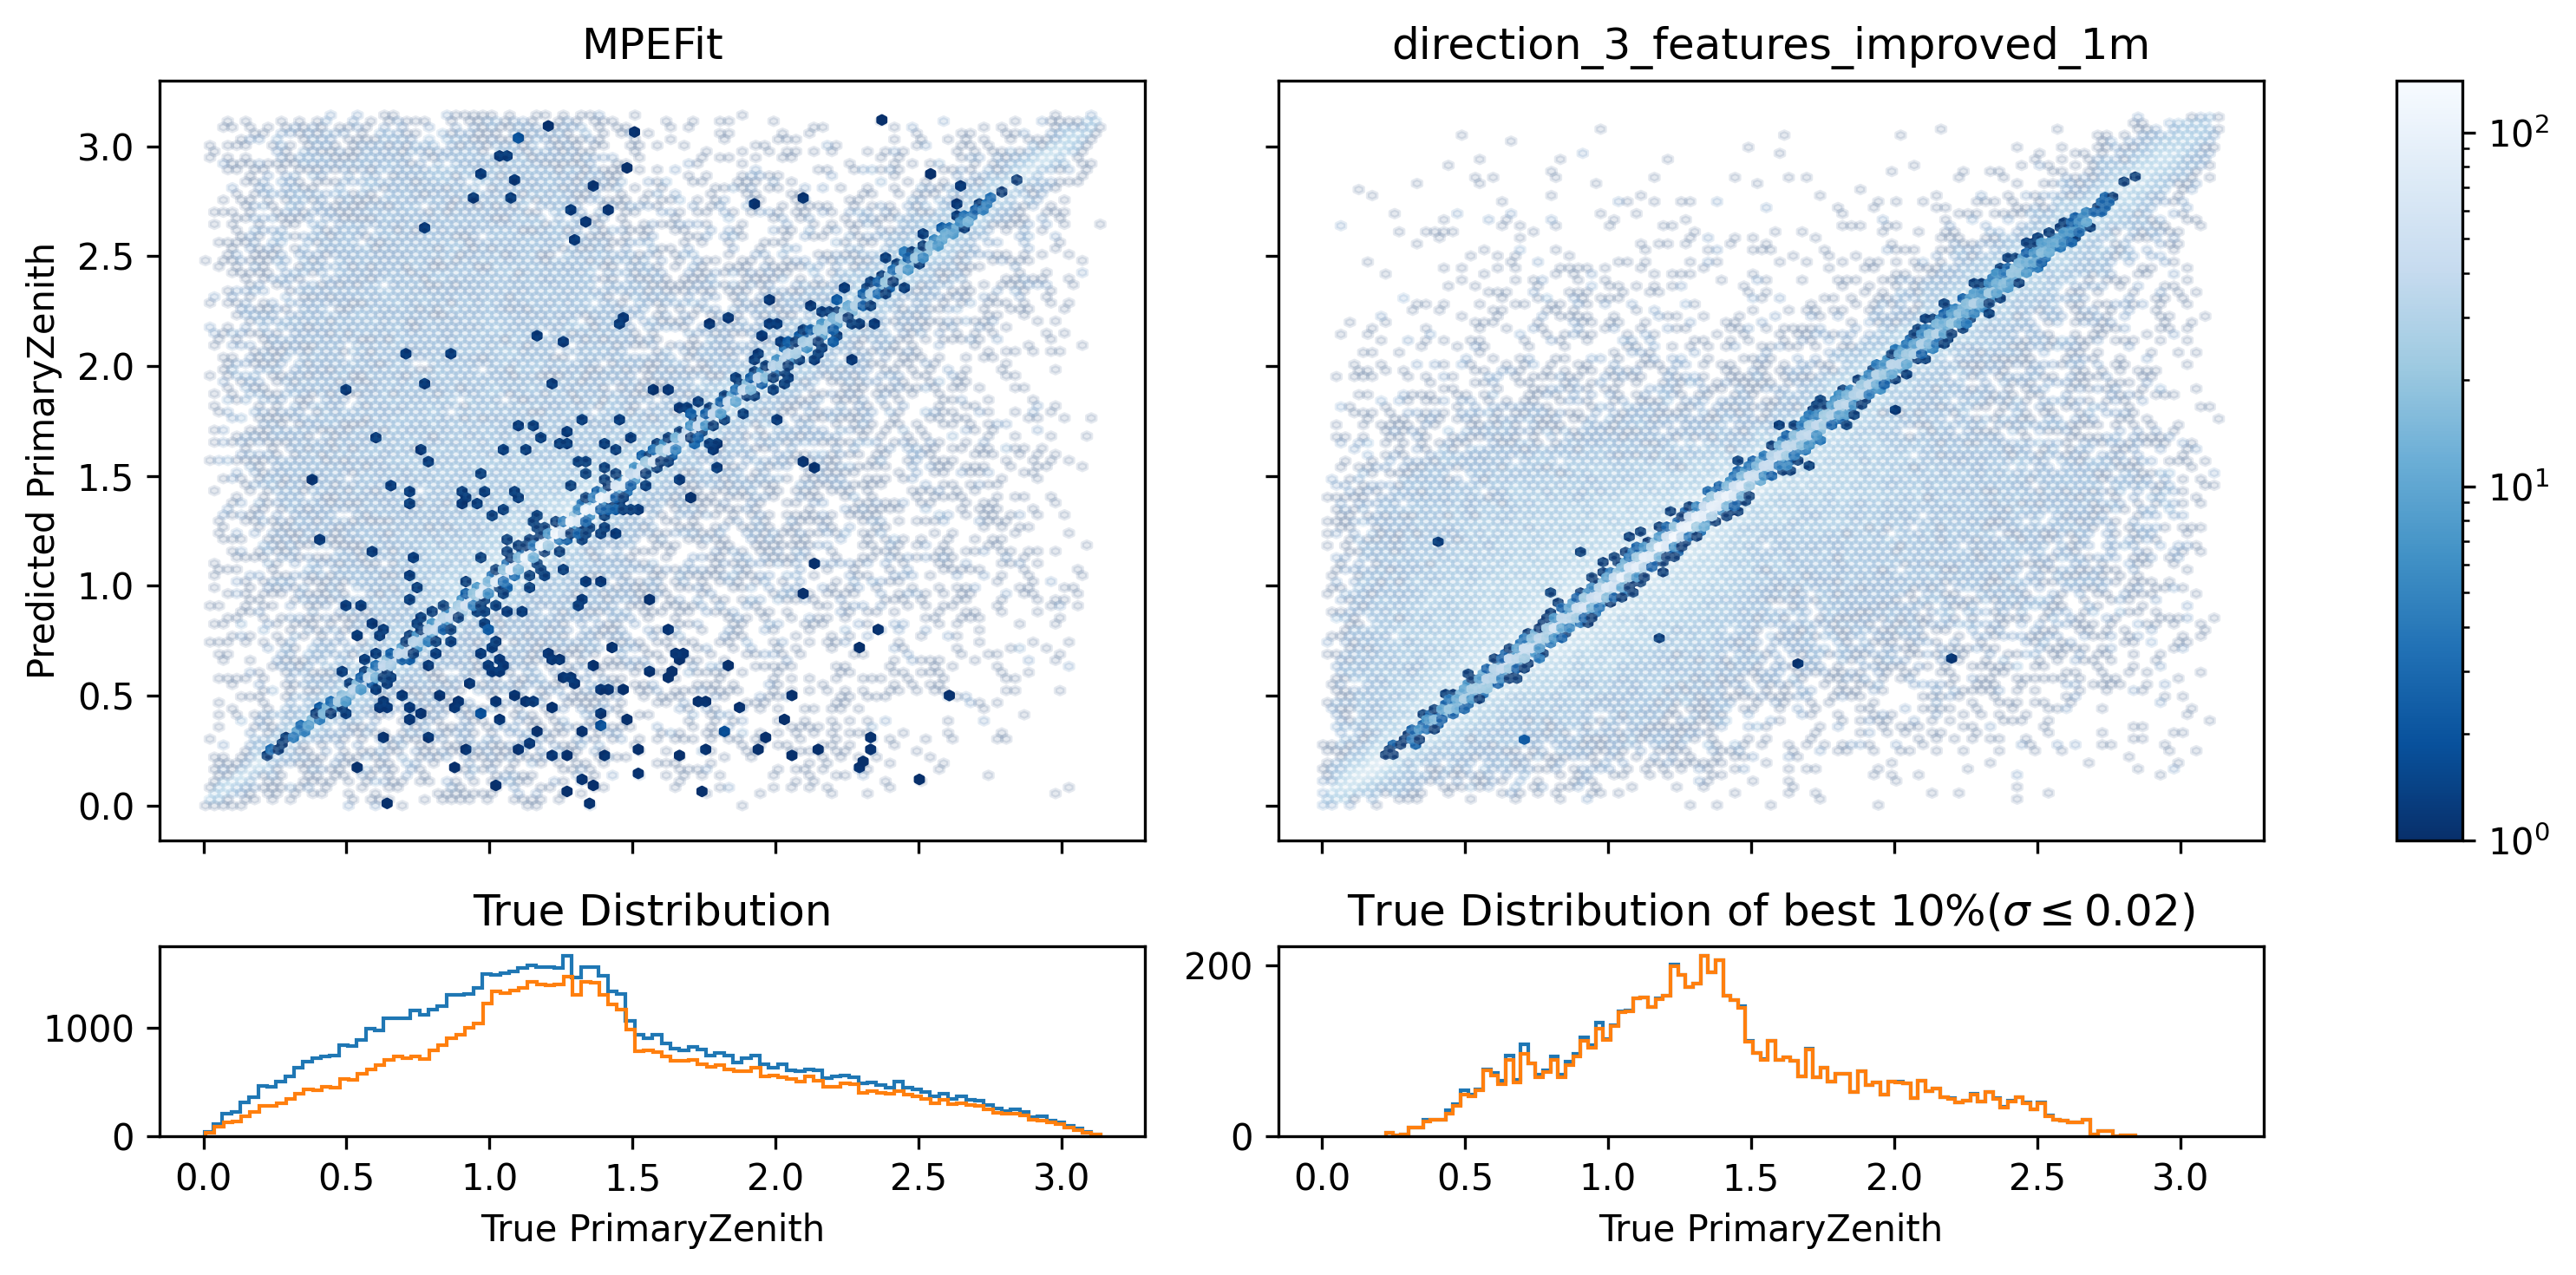
\includegraphics[width=.8\textwidth]{media/scatter_uncertainty_best.png}}
        \only<1>{\caption*{\small Hexagonal 2D-Bin plot in logarithmic color scale}}
        \only<2>{\caption*{\small Only showing 10\% of events with the lowest uncertainty estimate from DNN}}
    \end{figure}
\end{frame}